% !TEX root = waves.tex
\documentclass[a4paper,12pt]{report}
% Packages
%%%%%%%%%%%%%%%%%%%%%%%%%%%%%%%%%%%%%%%%%%%%%%%%%%%%%%%%%%%%%%%%%%%%%%%%%%%%%%
%% language, encoding & layout
\usepackage[british]{babel}
\usepackage[utf8]{inputenc}
\usepackage{mathpazo}
\usepackage{CrimsonPro}
\usepackage[T1]{fontenc}
\usepackage{xcolor}
\usepackage{microtype}
%% math symbols
\usepackage{amsmath,amssymb,braket,slashed,mathrsfs}
\usepackage[only,llbracket,rrbracket]{stmaryrd}
%% theorems
\usepackage{amsthm}
%% TikZ
\usepackage{tikz}
%% units
\usepackage[squaren,Gray,cdot,binary]{SIunits}
%% figures
\usepackage{graphicx}
\graphicspath{{./figures/}}
%% bibliography
\usepackage[square,authoryear]{natbib}
%% hyperlinks
\usepackage{hyperref}
\definecolor{linkcolor}{rgb}{.17578125,.1875,.5703125}
\hypersetup{
  pdfstartview={FitH},
  pdftitle={TITLE},
  pdfauthor={AUTHOR},
  pdfsubject={},
  pdfcreator={pdflatex},
  pdfkeywords={},
  colorlinks=true,
  linkcolor=linkcolor,
  citecolor=linkcolor,
  filecolor=black,
  urlcolor=linkcolor
}
%% compressed references
\usepackage{cleveref}
\newcommand{\crefrangeconjunction}{--}
%%% section
\crefformat{section}{Sec.~#2#1#3}
\crefmultiformat{section}{Sec.~#2#1#3}
{ and~#2#1#3}{, #2#1#3}{ and~#2#1#3}
\crefrangeformat{section}{Sec.~#3#1#4\,--\,#5#2#6}
%%% subsection
\crefformat{subsection}{Sec.~#2#1#3}
\crefmultiformat{subsection}{Sec.~#2#1#3}
{ and~#2#1#3}{, #2#1#3}{ and~#2#1#3}
\crefrangeformat{subsection}{Sec.~#3#1#4\,--\,#5#2#6}
%%% figure
\crefformat{figure}{Fig.~#2#1#3}
\crefmultiformat{figure}{Figs.~#2#1#3}
{ and~#2#1#3}{, #2#1#3}{ and~#2#1#3}
\crefrangeformat{figure}{Figs.~#3#1#4\,--\,#5#2#6}
%%% table
\crefformat{table}{Tab.~#2#1#3}
\crefmultiformat{table}{Tabs.~#2#1#3}
{ and~#2#1#3}{, #2#1#3}{ and~#2#1#3}
\crefrangeformat{table}{Tabs.~#3#1#4\,--\,#5#2#6}
%%% equation
\crefformat{equation}{Eq.~(#2#1#3)}
\crefmultiformat{equation}{Eqs.~(#2#1#3)}{ and~(#2#1#3)}{, (#2#1#3)}{ and~(#2#1#3)}
\crefrangeformat{equation}{Eqs.~(#3#1#4)--(#5#2#6)}
\graphicspath{{./figures/}}

% Header & footer
\usepackage[twoside]{fancyhdr}
\pagestyle{fancy}
\setlength{\headheight}{6mm}
\setlength{\headsep}{3mm}
\setlength{\footskip}{8mm}

% Page geometry
\usepackage[a4paper,left=25mm,right=25mm,top=20mm,bottom=20mm]{geometry}
\fancyhfoffset[E,O]{0pt} % recalculate the headers

% Theorem environments
%%%%%%%%%%%%%%%%%%%%%%%%%%%%%%%%%%%%%%%%%%%%%%%%%%%%%%%%%%%%%%%%%%%%%%%%%%%%%%
\theoremstyle{plain}
\newtheorem{theorem}{Theorem}[section]
\theoremstyle{plain}
\newtheorem{proposition}[theorem]{Proposition}
\theoremstyle{plain}
\newtheorem{corollary}[theorem]{Corollary}
\theoremstyle{plain}
\newtheorem{lemma}[theorem]{Lemma}
\theoremstyle{definition}
\newtheorem{definition}{Definition}[section]
\theoremstyle{definition}
\newtheorem{example}{Example}[section]
%%% cref labels
\crefformat{theorem}{Theorem~#2#1#3}
\crefformat{definition}{Definition~#2#1#3}
\crefformat{example}{Example~#2#1#3}

% New commands
%%%%%%%%%%%%%%%%%%%%%%%%%%%%%%%%%%%%%%%%%%%%%%%%%%%%%%%%%%%%%%%%%%%%%%%%%%%%%%
%% abbreviations
\newcommand{\cf}{{cf.}~}
\newcommand{\eg}{{e.g.}~}
\newcommand{\ie}{{i.e.}~}
%% math
\newcommand{\sq}{\mathrm{sq}}
\newcommand{\sw}{\mathrm{s}}
\newcommand{\cw}{\mathrm{c}}
\newcommand{\ew}{\mathrm{e}}
\newcommand{\diff}{\mathrm{d}}

% Title
%%%%%%%%%%%%%%%%%%%%%%%%%%%%%%%%%%%%%%%%%%%%%%%%%%%%%%%%%%%%%%%%%%%%%%%%%%%%%%
\title{Waves and Fourier analysis}
\author{Antonin Portelli}

% Document
%%%%%%%%%%%%%%%%%%%%%%%%%%%%%%%%%%%%%%%%%%%%%%%%%%%%%%%%%%%%%%%%%%%%%%%%%%%%%%
\begin{document}
\maketitle
%%%%%%%%%%%%%%%%%%%%%%%%%%%%%%%%%%%%%%%%%%%%%%%%%%%%%%%%%%%%%%%%%%%%%%%%%%%%%
\tableofcontents
\chapter{Elementary waves}
% !TEX root = ../waves.tex
%%%%%%%%%%%%%%%%%%%%%%%%%%%%%%%%%%%%%%%%%%%%%%%%%%%%%%%%%%%%%%%%%%%%%%%%%%%%%%%%%%%%%%%%%%
\section{Introduction: plucked strings}
As an introduction, we study a physical system which had a significant importance in the
historical development of Fourier analysis: the \emph{plucked string}. We consider in a
two-dimensional space a uniform string of length $L$ with linear mass density $\mu$ (in
$\kilogram\per\meter$), stretched between two points with coordinates $(0,0)$ and $(L,0)$.
We assume the string tension to be given by $T$ (in $\newton$). The action of plucking the
string consists in pulling it in a given position at time $t=0$, and releasing it. The
whole system is illustrated in~\cref{fig:string}. In the most general case, such system
can have a very complex behaviour, however we can introduce extra assumptions to simplify
it. We will assume in this section that we want to describe string vibrations for a
musical instrument, \eg an acoustic guitar. In this context, we clearly expect the string
oscillation to have an amplitude much smaller than the string length $L$.
\begin{figure}[t]
  \centering
  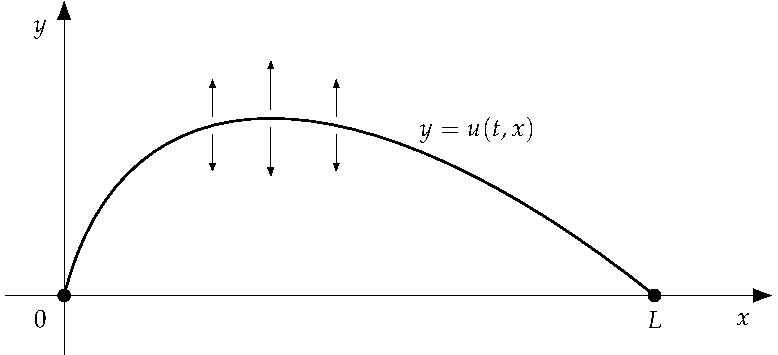
\includegraphics{tikz_string.pdf}
  \caption{Representation of the stretched string system. The arrows represent the
  transverse motion of the string.}
  \label{fig:string}
\end{figure}
%-----------------------------------------------------------------------------------------
\subsection{Derivation of the wave equation}
Let us apply the laws of mechanics to derive an equation describing the dynamics of this
system. We first start by approximating the string by a large number $N$ of elastic line
segments of equal mass $\epsilon\mu$, with $\epsilon=\frac{L}{N}$. The $n$-th segment on
the string has the end points $P_n=(x_n,y_n)$ and $P_{n+1}=(x_{n+1},y_{n+1})$, starting
from $P_0=(0,0)$ up to $P_N=(L,0)$. The continuous string dynamics will then be later
obtained through the $N\to+\infty$ limit, or equivalently $\epsilon\to 0$. We additionally
assume that each segment respond to the same tension $T$ at its end points. A view of the
vicinity of $n$-th segment is represented in~\cref{fig:string-inf}. We define the angle
$\theta_n$ between the $n$-th segment and the $x$-axis. At the point $P_n$, the total
force $\mathbf{F}_n$ is given by the tension forces from the neighbouring segments on the
string, explicitly
\begin{equation}
  \mathbf{F}_n=\mathbf{T}_n^-+\mathbf{T}_n^+\,,\label{eq:string-force}
\end{equation}
where the vectors $\mathbf{T}_n^\pm$ both have magnitude $T$ and are represented by the
blue arrows in~\cref{fig:string-inf}. Using the angles $\theta_n$ previously defined, the
coordinates of the tension forces are given by
\begin{align}
  \mathbf{T}_n^-&=-T(\cos(\theta_{n-1}),\sin(\theta_{n-1}))\,,\\
  \mathbf{T}_n^+&=T(\cos(\theta_{n}),\sin(\theta_{n}))\,.
\end{align}
Using Pythagoras' theorem and elementary trigonometry, one can write
\begin{align}
  \cos(\theta_n)&=\frac{x_{n+1}-x_n}{\sqrt{(x_{n+1}-x_n)^2+(y_{n+1}-y_n)^2}}\,,\\
  \sin(\theta_n)&=\frac{y_{n+1}-y_n}{\sqrt{(x_{n+1}-x_n)^2+(y_{n+1}-y_n)^2}}\,.
\end{align}
Defining the ratio $d_n=\smash{\frac{y_{n+1}-y_n}{x_{n+1}-x_n}}$, the expressions above
can be further simplified to
\begin{equation}
  \cos(\theta_n)=\frac{1}{\sqrt{1+d_n^2}}\qquad\text{and}\qquad
  \sin(\theta_n)=\frac{d_n}{\sqrt{1+d_n^2}}\,.
\end{equation}
Now, using Newton's Second Law with the total force~\cref{eq:string-force}, one obtains
the following system of differential of equations for the motion of $P_n$:
\begin{align}
  \epsilon\mu \frac{\diff^2 x_n}{\diff t^2}&=
  T\left(\frac{1}{\sqrt{1+d_{\smash{n+1}}^2}}-\frac{1}{\sqrt{1+d_{n}^2}}\right)\,,
  \label{eq:string-fullxeq}\\
  \epsilon\mu \frac{\diff^2 y_n}{\diff t^2}&=
  T\left(\frac{d_{n+1}}{\sqrt{1+d_{\smash{n+1}}^2}}-\frac{d_n}{\sqrt{1+d_{n}^2}}\right)\,.
  \label{eq:string-fullyeq}
\end{align}
This is a rather non-trivial system of coupled non-linear differential equations, and we
will now use our small amplitude assumption to simplify it. This approximation means that
the vertical distances $y_{n+1}-y_n$ are expected to be much smaller than the horizontal
ones $x_{n+1}-x_n$, or in other words, $d_n$ is close to zero. Let us then
expand~\cref{eq:string-fullxeq,eq:string-fullyeq} for $d_n\to 0$. We first remind the
Taylor expansion
\begin{equation}
  \frac{1}{\sqrt{1+x^2}}=1-\frac{x^2}{2}+\mathcal{O}(x^4)\,,
\end{equation}
leading to the leading-order approximation
\begin{align}
  \frac{\diff^2 x_n}{\diff t^2}&=0\,,\label{eq:string-loxeq}\\
  \frac{\diff^2 y_n}{\diff t^2}&=\frac{T}{\epsilon\mu}(d_{n+1}-d_n)\,,\label{eq:string-loyeq}
\end{align}
which is valid up to $\mathcal{O}(d_n^2)$ corrections. One remarkable feature of this
system is the fact that there is no force applying in the $x$ direction at leading order.
Since we assumed the string to be attached at its end points, this implies that there is
no motion in the $x$ direction. Oscillations in the $x$ and $y$ directions are called
\emph{longitudinal} and \emph{transverse} oscillations, respectively. We just obtained a
well-known result for string oscillations: in the limit of small oscillations, only
transverse oscillations are present.
\begin{figure}[t]
  \centering
  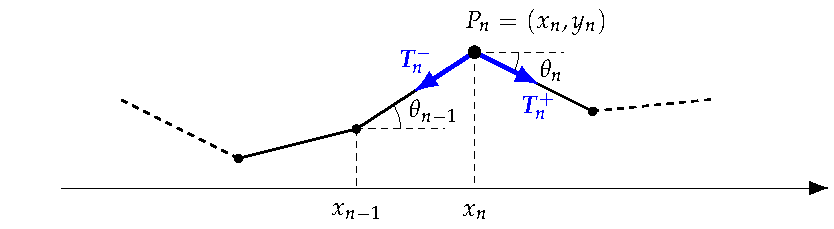
\includegraphics{tikz_string-inf.pdf}
  \caption{Discrete view of the string geometry and forces. The blue arrows represent the
  individual tension forces at point $P_n$.}
  \label{fig:string-inf}
\end{figure}

With the observation above, we can now exclusively focus on solving the transverse
equation of motion~\cref{eq:string-loyeq}. We assumed the string to have a uniform mass
distribution, and since the $x_n$ coordinates are constant and divide the string in
segments of equal mass, for all $n$ one has
\begin{equation}
  x_{n+1}-x_n=\epsilon\,.
\end{equation}
We additionally define the coordinates $y_n$ to be represented by a smooth function $u$ of
$x_n$ and the time $t$:
\begin{equation}
  y_n=u(t,x_n)\,.
\end{equation}
Substituting the equations above in~\cref{eq:string-loyeq}, one obtains
\begin{equation}
  \pdn{u}{t}{2}(t,x_n)=\frac{T}{\epsilon^2\mu}
  [u(t,x_{n}+\epsilon)-2u(t,x_{n})+u(t,x_{n}-\epsilon)]\,.\label{eq:wave-eq-discrete}
\end{equation}
We are now ready to obtain the continuous string equation by taking the $\epsilon\to 0$
limit. One starts by writing the Taylor expansion
\begin{equation}
  u(t,x+\epsilon)=u(t,x)+\epsilon\,\pd{u}{x}(t,x)
  +\frac{\epsilon^2}{2}\pdn{u}{x}{2}(t,x)+\mathcal{O}(\epsilon^3)\,,
\end{equation}
which implies that
\begin{equation}
  \lim_{\epsilon\to 0}=\frac{1}{\epsilon^2}
  [u(t,x+\epsilon)-2u(t,x)+u(t,x-\epsilon)]=\pdn{u}{x}{2}(t,x)\,.
\end{equation}
Using this last step with~\cref{eq:wave-eq-discrete} leads us to the main result of this
section, the \emph{wave equation}
\begin{equation}
  \boxed{
    \pdn{u}{t}{2}=c^2\,\pdn{u}{x}{2}
    \qquad\text{with}\qquad
  c=\sqrt{\frac{T}{\mu}}\,.}
  \label{eq:wave-eq}
\end{equation}
The parameter $c$, which has dimensions $\mathrm{L}\mathrm{T}^{-1}$, is usually called the
\emph{wave speed} for reasons that will be clear later in this section. The wave equation
is a homogeneous second-order partial differential equation, and will now discuss how to
solve it for the plucked string problem.
%-----------------------------------------------------------------------------------------
\subsection{General solutions of the wave equation}
We will first derive the general form of the solutions of the wave
equation~\cref{eq:wave-eq}. This derivation was first written by Jean le Rond d'Alembert
in 1747. \cref{eq:wave-eq} can be rewritten as follows
\begin{equation}
  \left(\pdn{}{t}{2}-c^2\,\pdn{}{x}{2}\right)u=
  \left(\pd{}{t}-c\,\pd{}{x}\right)
  \left(\pd{}{t}+c\,\pd{}{t}\right)u=0\,,
  \label{eq:wave-eq-factor}
\end{equation}
which is the composition of two first order derivatives. From this form, we would like to
define new length variables $\eta$ and $\xi$ such that
\begin{align}
  c\pd{}{\eta}&=\pd{}{t}+c\,\pd{}{x}\,,\\
  c\pd{}{\xi}&=\pd{}{t}-c\,\pd{}{x}\,.
\end{align}
Using the chain rules, we know that
\begin{align}
  \pd{}{\eta}&=\pd{t}{\eta}\pd{}{t}+\pd{x}{\eta}\pd{}{x}\,,\\
  \pd{}{\xi}&=\pd{t}{\xi}\pd{}{t}+\pd{x}{\xi}\pd{}{x}\,\,,
\end{align}
which implies that
\begin{equation}
  \pd{t}{\eta}=\frac{1}{c},\qquad\pd{x}{\eta}=1,\qquad
  \pd{t}{\xi}=\frac{1}{c},\qquad\text{and}\qquad\pd{x}{\xi}=-1\,.
\end{equation}
It is now clear that
\begin{align}
  t&=\frac{1}{c}(\eta+\xi)\,,\\
  x&=\eta-\xi\,,
\end{align}
is a possible solution, which can be inverted to
\begin{align}
  \eta&=x+ct\,,\\
  \xi&=x-ct\,.
\end{align}
In these new variables, the wave equation~\cref{eq:wave-eq-factor} becomes
\begin{equation}
  \frac{\partial^2 u}{\partial\eta\partial\xi}=0\,.
\end{equation}
In this simpler form, we can integrate the two derivatives sequentially. Starting with the
derivative in $\eta$, the right-hand side of the equation being zero means that
$\smash{\pd{u}{\xi}}$ is a constant in $\eta$. However, this constant can vary for any
value of $\xi$. In other words, there exists a function of one variable $\phi$ such that
\begin{equation}
  \pd{}{\xi}u(\eta,\xi)=\phi(\xi)\,.
\end{equation}
Following the same logic, as a function of $\xi$, $u$ is therefore an antiderivative of
$\phi$ up to a constant, which can vary with $\eta$. Therefore, there exists two functions
of a single variable $f$ and $g$ such that
\begin{equation}
  u(\eta,\xi)=f(\xi)+g(\eta)\,,
\end{equation}
where here $f$ is such that $f'=\phi$. In conclusion, switching back to the original
variables $x$ and $t$, the general solutions of the wave equation have the form
\begin{equation}
  \boxed{u(t,x)=f(x-ct)+g(x+ct)\,,}\label{eq:wave-eq-sol}
\end{equation}
where $f$ and $g$ can be any twice-differentiable functions. $f$ and $g$ are called the
\emph{forward-travelling} and \emph{backward-travelling} components, respectively. These
functions are named in this way for the following reason. At $t=0$, if one pick a point on
the curve of $f$ with $x$-coordinate $x_0$, then at an arbitrary time $t$ the same point
will have the $x$-coordinate
\begin{equation}
  x(t)=x_0+ct\,,
\end{equation}
\ie it is moving forward on the $x$ axis. Also, one notices that $\td{x}{t}=c$, meaning
the point is moving with speed $c$, justifying the name \emph{wave speed} introduced
earlier. The same observation can be made for $g$, moving backward on the $x$ axis.

As we can see, the space of solutions of the wave equation is very large as both forward
and backward contribution are arbitrary functions. However, it is known, and will be
admitted here, that the wave equation has a unique solution if one impose the two initial
conditions
\begin{equation}
  u_0(x)=u(0,x)\qquad\text{and}\qquad u_1(x)=\pd{u}{t}(0,x)\,,\label{eq:wave-eq-ic}
\end{equation}
which physically represent the initial position of the string and its initial velocity,
respectively. With this in mind, we will now discuss the solution of the wave equations
specifically for the plucked string problem.
%-----------------------------------------------------------------------------------------
\subsection{Particular solutions of the plucked string problem}
We remind here the considered physical problem: the string will be pulled in a given
position, and then released. This means the initial velocity $u_1$ in~\cref{eq:wave-eq-ic}
is zero. Without specifying, for the moment, the initial position, let us discuss what
this first initial condition implies. Coming back to the general
solution~\cref{eq:wave-eq-sol}, $u_1=0$ implies that for all $x$,
\begin{equation}
  u_1(x)=c[g'(x)-f'(x)]=0\,,
\end{equation}
which means that $f'=g'$. Two functions with equal derivatives differ by a unique
constant, so there is a unique real number $K$ such that $g(x)=f(x)+K$ for all $x$. So the
general solution of the wave equation becomes
\begin{equation}
  u(t,x)=f(x-ct)+f(x+ct)+K\,,
\end{equation}
and in particular the initial position is
\begin{equation}
  u_0(x)=2f(x)+K\,.\label{eq:u0K}
\end{equation}
Now, we can use the fact that the string is attached at the two points $(0,0)$ and
$(L,0)$, this implies that for all $t$
\begin{equation}
  u(t,0)=0\qquad\text{and}\qquad u(t,L)=0\,.
\end{equation}
These constraints are called the \emph{boundary conditions} of the wave equation, and they
generally have a strong influence on the set of solutions. Applying the boundary
conditions to~\cref{eq:u0K} directly implies that $K=0$. Let us now choose the initial
position of the string
%%%%%%%%%%%%%%%%%%%%%%%%%%%%%%%%%%%%%%%%%%%%%%%%%%%%%%%%%%%%%%%%%%%%%%%%%%%%%%%%%%%%%%%%%%
\section{Mathematical parametrisation of waves}
%%%%%%%%%%%%%%%%%%%%%%%%%%%%%%%%%%%%%%%%%%%%%%%%%%%%%%%%%%%%%%%%%%%%%%%%%%%%%%%%%%%%%%%%%%
\section{General properties of periodic functions}
A physical quantity $f(t)$ depending on a variable $t$ is said to be \emph{oscillating} or
\emph{periodic} if it repeats itself identically after a certain duration. In mathematical
terms:
\begin{definition}
  A function $f(t)$ is said to be~\emph{periodic} if there exists $T>0$ such that
  \begin{equation}
    \forall t,\quad f(t+T)=f(t)\,.
  \end{equation}
  $T$ is called a \emph{period} of $f(t)$.
\end{definition}
\noindent For example, $\sin(t)$ is periodic with period $2\pi$, and a constant function
admit any number has a period. Another fundamental quantity is the \emph{frequency}:
\begin{definition}
  If $T$ is a period of a given periodic function $f(t)$, its inverse
  \begin{equation}
    \omega=\frac{1}{T}
  \end{equation}
  is called a \emph{frequency} of $f(t)$.
\end{definition}
\noindent In physical terms, if $t$ is a time variable, $T$ is also a time, and $\omega$
is the number of oscillations per unit of time. One can notice that a periodic function
never has a unique period, \eg clearly if $T$ is a period, $2T$ is also a period. Because
of this it is useful to write the following definition
\begin{definition}
  The infimum $T_0$ of the set of all possible periods of a given periodic function $f(t)$
  is called the \emph{fundamental period} of $f(t)$. The associated frequency
  $\omega_0=\frac{1}{T_0}$ is called the \emph{fundamental frequency} of $f(t)$.
\end{definition}
\noindent For example, the fundamental frequency of $\sin(t)$ is $2\pi$, and it is zero
for a constant function. Another fundamental quantity is the \emph{amplitude} of a
periodic function, measuring the size of the oscillations within a fundamental period:
\begin{definition}
  \label{def:amplitude}
  Let $f(t)$ be a real periodic function with fundamental period $T_0$. We additionally
  assume that $f(t)$ is bounded with infimum and supremum
  \begin{equation}
    m=\inf_{0\leq t\leq T_0}f(t)\qquad\text{and}\qquad M=\sup_{0\leq t\leq T_0}f(t)\,.
  \end{equation}
  The \emph{amplitude} of $f(t)$ is then defined by
  \begin{equation}
    A=\frac{M-m}{2}\,.
  \end{equation}
\end{definition}
\noindent For example, the amplitude of $\sin(t)$ is equal to $1$, and it is zero for
constant functions. \cref{def:amplitude} assumes that $f(t)$ is bounded, and one can
question whether this hypothesis is true in general. It is not, but continuity is a
sufficient condition:
\begin{proposition}
  If a real periodic function is continuous, then it is bounded (and therefore it has a
  well-defined amplitude).
\end{proposition}
\begin{proof}
  Let $f(t)$ be a continuous periodic function with fundamental period $T_0$. Since $f(t)$
  is continuous on the compact interval $[0,T_0]$, it follows from the boundedness theorem
  that it is also bounded on this interval. Finally, using the periodicity, any value
  $f(t)$ is equal to a value $f(t_0)$ with $0\leq t_0\leq T$, therefore $f(t)$ is bounded.
\end{proof}
\noindent One can show that this condition is not necessary, \ie discontinuous periodic
functions can be bounded as well. One example of such function is the \emph{square wave},
that will be useful later:
\begin{definition}
  \label{def:sq-wave}
  The square wave function $\sq(t)$ is defined by
  \begin{equation}
    \sq(t)=
    \begin{cases}
      1, &\text{if~}\lfloor 2t\rfloor~\text{is even}\\
      -1, &\text{if~}\lfloor 2t\rfloor~\text{is odd}\\
    \end{cases}\,,
  \end{equation}
  where $\lfloor t\rfloor$ is the floor function, \ie the largest integer smaller or equal
  to $t$.
\end{definition}
\noindent It is left as an exercise to the reader to show that $\sq(t)$ is periodic with
fundamental period $1$ and amplitude $1$, and can be rewritten as
\begin{equation}
  \sq(t)=2(2\lfloor t\rfloor-\lfloor 2t\rfloor)+1\,.
\end{equation}
Additionally, $\sq(t)$ is discontinuous at all points of the form $\frac{n}{2}$ where
$n\in\mathbb{Z}$. The curve of $\sq(t)$ is represented in~\cref{fig:sq-wave}.
\begin{figure}[t]
  \centering
  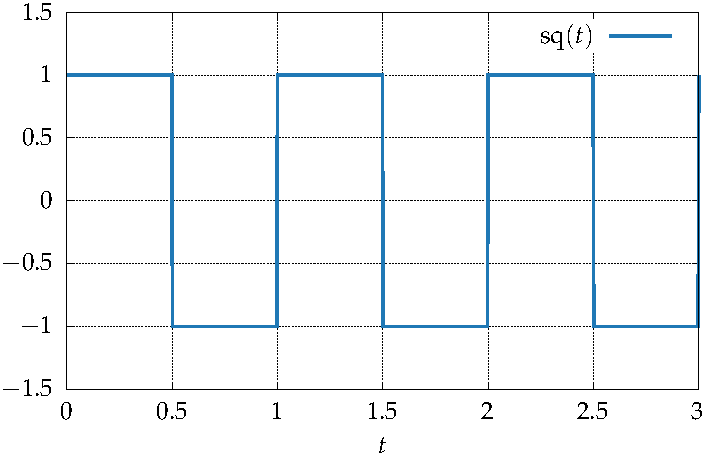
\includegraphics{gp_sq-wave.pdf}
  \caption{Curve of the square wave defined in~\cref{def:sq-wave}.}
  \label{fig:sq-wave}
\end{figure}
As mentioned above, the sine function provides a way to construct explicit examples of
periodic functions. We will see that it is, in fact, a fundamental building block of
periodic functions, which is the essence of Fourier analysis. It is therefore useful to
familiarise beforehand with periodic functions built using the sine function.
%%%%%%%%%%%%%%%%%%%%%%%%%%%%%%%%%%%%%%%%%%%%%%%%%%%%%%%%%%%%%%%%%%%%%%%%%%%%%%%%%%%%%%%%%%
\section{Elementary waves}
We start by defining elementary sine waves
\begin{definition}
  We call \emph{elementary sine wave} the function defined by
  \begin{equation}
    \sw(t;\omega,\phi)=\sin(2\pi\omega t + \phi)\,.\label{eq:sine-wave}
  \end{equation}
  where $\omega\geq 0$ and $0\leq\phi<2\pi$ are the \emph{frequency} and \emph{phase} of
  the wave, respectively. When the phase argument is omitted then it is assumed that
  $\phi=0$, \ie $\sw(t;\omega)=\sw(t;\omega,0)$.
\end{definition}
\noindent It is straightforward to show that, according to the definition in the previous
section, $\sw(t;\omega,\phi)$ is a periodic function with fundamental frequency $\omega$
and amplitude $1$. The phase measures the delay in the oscillation relatively to a wave
with identical frequency equal to zero at $t=0$. More generally if two waves have
identical frequencies and different phases $\phi_1$ and $\phi_2$, the time delay between
them is given by
\begin{equation}
  \delta t =\frac{T}{2\pi}\delta\phi\qquad\text{with}\qquad\delta\phi=\phi_1-\phi_2\,,
\end{equation}
explicitly
\begin{equation}
  \sw(t;\omega,\phi_1)=\sw(t+\delta t;\omega,\phi_2)\,.
\end{equation}
In other words, the phase can always be re-written as a shift in time:
\begin{equation}
  \sw(t;\omega,\phi)=\sw(t+t_0;\omega),
  \qquad\text{with}\qquad
  t_0 = \frac{T\phi}{2\pi}\,.\label{eq:phase-delay}
\end{equation}
The frequency and phase are represented graphically in~\cref{fig:sine-wave}.
\begin{figure}[t]
  \centering
  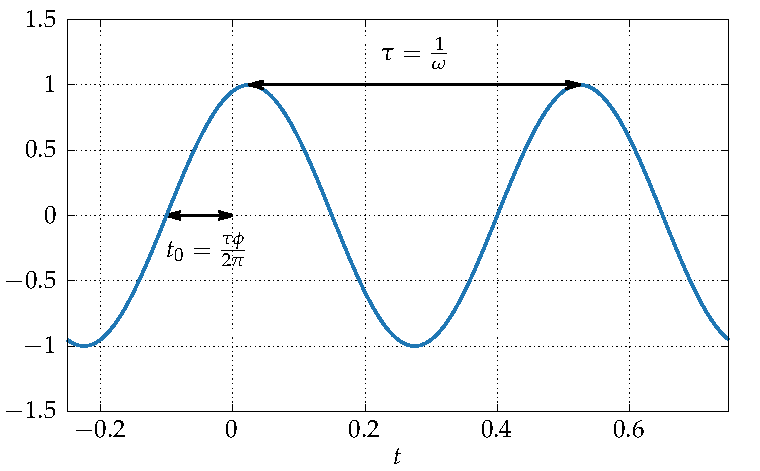
\includegraphics{gp_sine-wave.pdf}
  \caption{Example curve of the sine wave defined in~\cref{eq:sine-wave}, with frequency
    $\omega=2$ and phase $\phi=0.2\times 2\pi$. The arrows represent the period
  $T=\frac{1}{\omega}$ and the phase delay from~\cref{eq:phase-delay}.}
  \label{fig:sine-wave}
\end{figure}

For the special phase $\frac{\pi}{2}$, a sine wave can be written using the cosine
function:
\begin{equation}
  \sw\left(t;\omega,\frac{\pi}{2}\right)= \cos(2\pi\omega t)\,,
\end{equation}
motivating the following definition
\begin{definition}
  We call \emph{elementary cosine wave} the function
  \begin{equation}
    \cw(t;\omega,\phi)=\cos(2\pi\omega t + \phi)\,.\label{eq:cosine-wave}
  \end{equation}
  Similarly to the case of sine waves we define $\cw(t;\omega)=\cw(t;\omega,0)$. Sine and
  cosine waves are related by the following trivial relationships
  \begin{equation}
    \sw(t;\omega,\phi)=\cw\left(t;\omega,\phi-\frac{\pi}{2}\right),
    \quad\text{and}\quad
    \cw(t;\omega,\phi)=\sw\left(t;\omega,\phi+\frac{\pi}{2}\right)\,.
  \end{equation}
\end{definition}

A crucial set of formula to manipulate waves is given by the following angle addition
theorem:
\begin{theorem}[Angle addition]
  \label{thm:angle-add}
  For all pairs of real numbers $a$ and $b$, one has the following identities
  \begin{align}
    \sin(a+b)&=\sin(a)\cos(b)+\cos(a)\sin(b)\,,\label{eq:sinapb}\\
    \sin(a-b)&=\sin(a)\cos(b)-\cos(a)\sin(b)\,,\label{eq:sinamb}\\
    \cos(a+b)&=\cos(a)\cos(b)-\sin(a)\sin(b)\,,\label{eq:cosapb}\\
    \cos(a-b)&=\cos(a)\cos(b)+\sin(a)\sin(b)\,.\label{eq:cosamb}
  \end{align}
\end{theorem}
\begin{proof}
  We remind that the sine and cosine function are the real and imaginary part of complex
  exponential
  \begin{equation}
    e^{i\theta}=\cos(\theta)+i\sin(\theta)\,.
  \end{equation}
  Therefore,
  \begin{equation}
    e^{i a}e^{i b}=\cos(a)\cos(b)-\sin(a)\sin(b)+i[\cos(a)\sin(b)+\sin(a)\cos(b)]\,,\label{eq:eaeb}
  \end{equation}
  and by definition
  \begin{equation}
    e^{i(a+b)}=\cos(a+b)+i\sin(a+b)\,.\label{eq:eapb}
  \end{equation}
  Now, using the fact that $e^{i(a+b)}=e^{i a}e^{i b}$, and identifying the real and
  imaginary parts in~\cref{eq:eaeb,eq:eapb}, one directly
  obtains~\cref{eq:sinapb,eq:cosapb}. \cref{eq:sinamb,eq:cosamb} can then be obtained
  using the parity properties of the sine and cosine functions, namely $\sin(-x)=-\sin(x)$
  and $\cos(-x)=\cos(x)$.
\end{proof}
The angle addition theorem can be proven solely using triangle geometry, which is
significantly less trivial than the simple proof above based on complex numbers. More
generally, elementary waves are indeed easier to manipulate using complex exponentials,
motivating the definition below.
\begin{definition}
  We call \emph{elementary complex wave} the function
  \begin{equation}
    \ew(t;\omega,\phi)=e^{i(2\pi\omega t + \phi)}\,.
  \end{equation}
  As previously we define $\ew(t;\omega)=\ew(t;\omega,0)$. By definition of the complex
  exponential, elementary complex waves are related to sine and cosine elementary waves by
  the relation
  \begin{equation}
    \ew(t;\omega,\phi)=\cw(t;\omega,\phi)+i\,\sw(t;\omega,\phi)\,,
  \end{equation}
  Thanks to the properties of the exponential, we have the two following trivial
  relationships
  \begin{equation}
    \ew(t;\omega,\phi)=e^{i\phi}\ew(t;\omega)\,\quad\text{and}\quad
    \ew(t;\omega,\phi)^*=\ew(-t;\omega,-\phi)=\ew(t;-\omega,-\phi)\,,\label{eq:cw-conj}
  \end{equation}
  where $z^*$ is the conjugate of the complex number $z$. Using these formulas, the
  relationship to sine and cosine waves can be rewritten as
  \begin{align}
    \cw(t;\omega,\phi)&=\frac{1}{2}[\ew(t;\omega,\phi)+\ew(t;-\omega,-\phi)]\,,
    \label{eq:cwtoew}\\
    \sw(t;\omega,\phi)&=-\frac{i}{2}[\ew(t;\omega,\phi)-\ew(t;-\omega,-\phi)]\,.
    \label{eq:swtoew}
  \end{align}
\end{definition}

A considerable simplification with complex waves comes from the fact that the phase is
just a multiplicative factor, equivalent to giving a \emph{complex amplitude} to the wave.
Similarly, phased sine and cosine waves can be expressed as a sum of zero-phase ones using
the angle addition theorem:
\begin{align}
  \sw(t;\omega,\phi)&=\cos(\phi)\sw(t;\omega)+\sin(\phi)\cw(t;\omega)\,,\\
  \cw(t;\omega,\phi)&=\cos(\phi)\cw(t;\omega)-\sin(\phi)\sw(t;\omega)\,.
\end{align}

%%%%%%%%%%%%%%%%%%%%%%%%%%%%%%%%%%%%%%%%%%%%%%%%%%%%%%%%%%%%%%%%%%%%%%%%%%%%%%%%%%%%%%%%%%
\section{Combination of elementary waves}
We will now discuss how to create more general waves by adding elementary waves. One first
legitimate question is whether the sum of two periodic functions is till periodic. It is
not always true, and can be characterised by the following result:
\begin{theorem}
  \label{thm:period-sum}
  Let $f_1(t)$ and $f_2(t)$ be two periodic functions of fundamental periods $T_1\neq 0$
  and $T_2\neq 0$, respectively. Then, for any pair of non-zero complex numbers $\alpha_1$
  and $\alpha_2$, the linear combination
  \begin{equation}
    f(t)=\alpha_1 f_1(t)+\alpha_2 f_2(t)
  \end{equation}
  is periodic if and only if the period ratio  $\frac{T_1}{T_2}$ is a rational number. If
  this condition is true, this ratio can be written $\frac{T_1}{T_2}=\frac{p}{q}$ where
  $p$ and $q$ are two coprime integers (\ie their GCD is $1$), and the fundamental
  frequency $T$ of $f(t)$ is given by
  \begin{equation}
    T=qT_1=pT_2\,.
  \end{equation}
\end{theorem}
\begin{example}
  \label{ex:period-sum}
  $\sin\left(\frac{2\pi}{3}t\right)+\sin(\pi t)$ is periodic with fundamental period $6$.
\end{example}
\begin{example}
  \label{ex:nperiod-sum}
  $\sin(t)+\sin(\pi t)$ is not periodic.
\end{example}
\noindent Both examples above are illustrated in~\cref{fig:sine-sum}. Mathematically
speaking,~\cref{thm:period-sum} means that generally periodic functions sums are not
periodic. However, we remind that any real number is arbitrarily close to a rational
number, so non-periodic sums like in~\cref{ex:nperiod-sum} can always be approximated
arbitrarily well by a periodic function. This is relevant for physics and engineering
applications where quantities are often known up to some limited precision.
\begin{figure}[t]
  \centering
  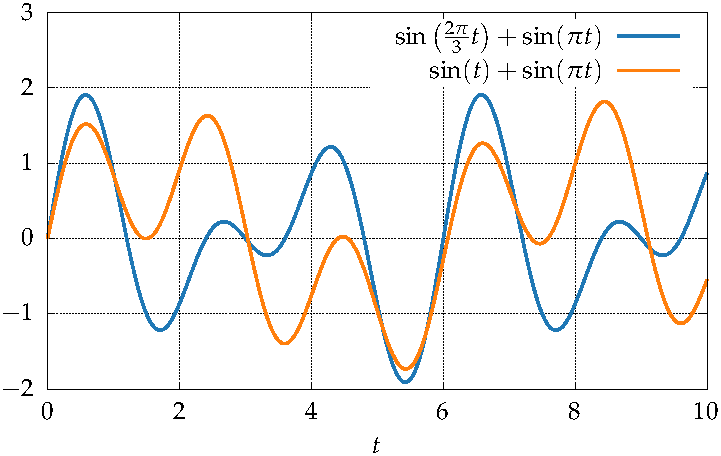
\includegraphics{gp_sine-sum.pdf}
  \caption{Curves of the sine wave sums in~\cref{ex:period-sum,ex:nperiod-sum}}
  \label{fig:sine-sum}
\end{figure}

Based on the theorem above, we can make the following definition for an arbitrary linear
combination of elementary waves:
\begin{definition}
  We call \emph{trigonometric polynomial} of degree $N$ and frequency $\omega$ any
  function of the form
  \begin{equation}
    P(t)=a_0+\sum_{n=1}^N[a_n\,\cw(t;n\omega)+b_n\,\sw(t;n\omega)]\,,
    \label{eq:trigp-sc}
  \end{equation}
  where $a_n$ and $b_n$ are real coefficients such that $a_N\neq 0$ or $b_N \neq 0$. The
  formula above is called the \emph{sine-cosine form} of $P(t)$ with \emph{sine-cosine
  coefficients} or \emph{modes} $a_n$ and $b_n$.
\end{definition}
It is clear that such function is periodic, and a consequence of~\cref{thm:period-sum} is
then
\begin{proposition}
  Let $P$ be a trigonometric polynomial of degree $N\geq 1$ and frequency $\omega$ with
  sine-cosine coefficients $a_n$ and $b_n$. $P$ is a periodic function with period
  $T=\frac{1}{\omega}$, and additionally if $a_1\neq0$ or $b_1\neq0$, then $\omega$ is the
  fundamental frequency of $P(t)$.
\end{proposition}
\begin{proof}
  Each term in~\cref{eq:trigp-sc} is trivially $T$-periodic, so $P$ is also $T$-periodic.
  Now, the $n$-th mode of $P$ has a fundamental period of $T_n=\frac{T}{n}$. Assuming that
  $a_1\neq0$ or $b_1\neq0$, then the period ratio of this first mode to an arbitrary
  non-vanishing higher mode $n$ is given by
  \begin{equation}
    \frac{T_1}{T_n}=n\,.
  \end{equation}
  Using~\cref{thm:period-sum}, this means that this combination of modes has fundamental
  period $T$. The remaining modes can then be added one after another, and repeated use
  of~\cref{thm:period-sum} demonstrate the proposition.
\end{proof}
As we previously did for the elementary waves, trigonometric polynomials can be put in a
more convenient complex form
\begin{definition}
  \label{def:trigp-complex}
  Let $P$ be a trigonometric polynomial of degree $N$ and frequency $\omega$ with
  sine-cosine coefficients $a_n$ and $b_n$. $P$ can be written in the \emph{complex form}
  \begin{equation}
    P(t)=\sum_{n=-N}^{N}c_n\ew(t;n\omega)\,,\label{eq:trigp-complex}
  \end{equation}
  with the \emph{complex coefficients}
  \begin{equation}
    c_n =
    \begin{cases}
      a_0 &\text{if~}n=0\\
      \frac{1}{2}(a_n-ib_n)&\text{if~}n>0\\
      \frac{1}{2}(a_n+ib_n)&\text{if~}n<0
    \end{cases}
    \,,\label{eq:ab-to-c}
  \end{equation}
  which have the property $c_n^*=c_{-n}$. The relation above can be inverted to
  \begin{equation}
    a_n=c_n+c_{-n}\qquad\text{and}\qquad
    b_n=i(c_n-c_{-n})\,.
  \end{equation}
\end{definition}
The formulas in the definition above can be obtained using~\cref{eq:cwtoew,eq:swtoew} with
the definition~\cref{eq:trigp-sc}, which is left as an exercise to the reader. A key
property of trigonometric polynomials, that will be crucial later, is the unicity of their
coefficients, formulated in the theorem below
\begin{theorem}
  \label{thm:trigp-unicity}
  Let $P$ and $Q$ be two trigonometric polynomials with the same frequency $\omega$,
  degrees $N$ and $N'$, and sine-cosine coefficients $a_n$,$b_n$ and $a'_n$,$b'_n$,
  respectively. $P$ and $Q$ are identically equal,~\ie $P(t)=Q(t)$ for all $t$, if and
  only if their degrees and coefficients are equal, \ie $N=N'$ and for all $n$
  \begin{equation}
    a_n=a'_n\quad\text{and}\quad b_n=b'_n\,.
  \end{equation}
\end{theorem}
Although we could attempt to prove that directly, this theorem is a consequence of a
fundamental orthogonality property of elementary waves which is crucial in Fourier
analysis. This will be the topic of the next section, where we will prove the theorem
above. Using the relationships in~\cref{def:trigp-complex}, \cref{thm:trigp-unicity}
directly implies that the complex coefficients are also unique.

We, so far, only considered linear combinations of elementary waves. We conclude this
section by looking at products of elementary waves, which thanks to the angle addition
theorem can be reduced to linear combinations:
\begin{proposition}
  The following identities hold for multiplying elementary waves:
  \begin{align}
    \cw(\omega_1)\cw(\omega_2)&=\frac{1}{2}[\cw(\omega_1-\omega_2)+\cw(\omega_1+\omega_2)]
    \label{eq:cprod}\\
    \sw(\omega_1)\sw(\omega_2)&=\frac{1}{2}[\cw(\omega_1-\omega_2)-\cw(\omega_1+\omega_2)]
    \label{eq:sprod}\\
    \sw(\omega_1)\cw(\omega_2)&=\frac{1}{2}[\sw(\omega_1-\omega_2)+\sw(\omega_1+\omega_2)]
    \label{eq:scprod}\\
    \ew(\omega_1)\ew(\omega_2)&=\ew(\omega_1+\omega_2)\label{eq:eprod}
  \end{align}
\end{proposition}
\begin{proof}
  These identities are a trivial re-interpretation of~\cref{thm:angle-add}.
\end{proof}
%%%%%%%%%%%%%%%%%%%%%%%%%%%%%%%%%%%%%%%%%%%%%%%%%%%%%%%%%%%%%%%%%%%%%%%%%%%%%%%%%%%%%%%%%%
\section{Orthogonality of elementary waves}
In vector calculus, given an $n$-dimensional real vector $v$ and a unit vector $u$, the
\emph{orthogonal projection} $v_u$ of $v$ on the axis defined by $u$ is given by
\begin{equation}
  \label{eq:orth-proj}
  v_u=\cos(\theta)|v|\,u\,,
\end{equation}
where $\theta$ is the angle between $u$ and $v$, and $|v|$ is the norm of $v$. The
projection coefficient $\cos(\theta)|v|$ is known to be given by the \emph{dot product}
\begin{equation}
  v\cdot u=\sum_{j=1}^n v_j u_j=\cos(\theta)|v|\,.\label{eq:vec-dot}
\end{equation}
Additionally, the dot product $v\cdot u$ vanishes when $v$ and $u$ are \emph{orthogonal}
(\ie they form an angle of $\pi$ radians). This makes the dot product an essential tool of
vector calculus to compute the coordinate of vectors in an orthonormal basis. Explicitly,
let $e_j$ be an orthonormal basis of $\mathbb{R}^n$, and let $v^{e}_j$ be the coefficients
of $v$ in that basis, \ie
\begin{equation}
  v=\sum_{j=1}^{n}v^{e}_j\,e_j\,,
\end{equation}
then the $v^{e}_j$ can be computed using the dot product using
\begin{equation}
  v^{e}_j=v\cdot e_j\,.\label{eq:basis-proj}
\end{equation}
\begin{figure}[t]
  \caption{Visual representation of the orthogonal projection of a vector on a unit vector
  given in~\cref{eq:orth-proj}}
  \label{fig:orth-proj}
\end{figure}

The concept of orthogonality and orthogonal projection can be generalised to more complex
mathematical objects like functions. As demonstrated below, elementary waves can be
interpreted as an orthogonal basis for trigonometric polynomial, which is the reason
why~\cref{thm:trigp-unicity} holds, and a key structure at the heart of Fourier analysis.
Although the general description of orthogonality between functions is out of the scope of
this lecture and will not be treated here, this introduction to Fourier analysis can be
seen as a good introduction to this type of concept.

We start by defining the dot product between two periodic functions
\begin{definition}
  Let $f$ and $g$ two real $T$-periodic functions. We assume that $f$ and $g$ are
  integrable on the interval $[0,T]$. The \emph{dot product} $\braket{f,g}$ between $f$
  and $g$ is the real number defined by
  \begin{equation}
    \braket{f,g}=\int_{0}^{T}\diff t\, f(t)g(t)\,.\label{eq:func-dot}
  \end{equation}
  Additionally, the \emph{norm} $\|f\|$ of the function $f$ is defined by
  \begin{equation}
    \|f\|^2=\braket{f,f}=\int_{0}^{T}\diff t\, f(t)^2\,.
  \end{equation}
\end{definition}
The definition~\cref{eq:func-dot} can be interpreted as a continuous version
of~\cref{eq:vec-dot}, where the values $f(t)$ and $g(t)$ are the ``continuous
coordinates'' of the functions $f$ and $g$, and the integral is a ``continuous sum'' over
these coordinates\footnote{Expressions within quotes are meant to be understood
  intuitively, their precise mathematical definition is more challenging and out of scope
here.}. The functional dot product has the same linearity and commutativity properties
than the vector dot product:
\begin{proposition}
  Let $f$, $g$, and $h$ be three real $T$-periodic functions. The following identities
  hold for any pair of real number $\alpha$ and $\beta$
  \begin{align}
    \braket{\alpha f+\beta g,h}&=\alpha\braket{f,h}+\beta\braket{g,h}\,,\\
    \braket{f,\alpha g+\beta h}&=\alpha\braket{f,g}+\beta\braket{f,h}\,,\\
    \braket{f,g}&=\braket{g,f}\,.
  \end{align}
\end{proposition}
\begin{proof}
  This is a trivial consequence of the definition~\cref{eq:func-dot} and the linearity of
  the integral.
\end{proof}
The definition of orthogonality follows naturally:
\begin{definition}
  \label{def:dot-rfunc}
  Let $f$ and $g$ be two $T$-periodic functions. $f$ and $g$ are said to be
  \emph{orthogonal} if their dot product vanishes, \ie
  \begin{equation}
    \braket{f,g}=0\,.
  \end{equation}
\end{definition}
We now give the main result of this section, \ie the orthogonality of elementary waves
\begin{theorem}
  \label{thm:sc-orth}
  Let $\omega>0$ be an arbitrary frequency corresponding to the period $T$. For any pair
  of integers $n$ and $m$, the following identities hold
  \begin{align}
    \braket{\sw(n\omega),\sw(m\omega)}&=\frac{T}{2}\delta_{nm}\,,\label{eq:sw-orth}\\
    \braket{\cw(n\omega),\cw(m\omega)}&=\frac{T}{2}\delta_{nm}\,,\label{eq:cw-orth}\\
    \braket{\cw(n\omega),\sw(m\omega)}&=0\,.\label{eq:scw-orth}
  \end{align}
  Where $\delta_{nm}$ is the \emph{Kronecker symbol}
  \begin{equation}
    \delta_{nm}=
    \begin{cases}
      1&~\mathrm{if}~~n=m\\
      0&~\mathrm{else}
    \end{cases}\,.
  \end{equation}
  In other words, for any pair of integers $n$ and $m$, sine waves of the form
  $\sw(n\omega)$ and $\sw(m\omega)$ have norm squared $\frac{T}{2}$ and are orthogonal if
  and only if $n\neq m$, the same applies to cosine waves, and a sine and a cosine wave of
  the form $\sw(n\omega)$ and $\cw(m\omega)$ are always orthogonal.
\end{theorem}
\begin{proof}
  Let us demonstrate~\cref{eq:sw-orth,eq:cw-orth,eq:scw-orth} using the
  definition~\cref{eq:func-dot}. We start with~\cref{eq:sw-orth}
  \begin{equation}
    \braket{\sw(n\omega),\sw(m\omega)}=\int_{0}^{T}\diff t\,
    \sin(2\pi n\omega t)\sin(2\pi m\omega t)\,.
  \end{equation}
  Using~\cref{eq:sprod}, one has
  \begin{equation}
    \sw(n\omega)\sw(m\omega)=\frac{1}{2}\{\cw[(n-m)\omega]-\cw[(n+m)\omega]\}\,.
    \label{eq:sw-prod}
  \end{equation}
  If $n=m$, this product simplifies to
  \begin{equation}
    \sw(n\omega)\sw(m\omega)=\frac{1}{2}[1-\cw(2n\omega)]\,,
  \end{equation}
  which integrates to
  \begin{equation}
    \frac{1}{2}\int_{0}^{T}\diff t\,[1-\cos(4\pi n\omega t)]=\frac{T}{2}-
    \left[\frac{1}{8\pi n\omega}\sin(4\pi n\omega t)\right]_0^T
    =\frac{T}{2}\,.
  \end{equation}
  If $n\neq m$, \cref{eq:sw-prod} integrates to
  \begin{align}
    &\frac{1}{2}\int_{0}^{T}\diff t\,\{\cos[2\pi(n-m)\omega t]-\cos[2\pi(n+m)\omega t]\}\notag\\
    &\qquad\qquad=\left[\frac{1}{2\pi(n-m)\omega}\sin[2\pi(n-m)\omega t]
    -\frac{1}{2\pi(n+m)\omega}\sin[2\pi(n+m)\omega t]\right]_0^T\notag\\
    &\qquad\qquad=0
  \end{align}
  Both equations above demonstrate~\cref{eq:sw-orth}. We now turn to~\cref{eq:cw-orth}, we
  start by using the product identity~\cref{eq:cprod}
  \begin{equation}
    \cw(n\omega)\cw(m\omega)=\frac{1}{2}\{\cw[(n-m)\omega]+\cw[(n+m)\omega]\}\,,
  \end{equation}
  which is identical to~\cref{eq:sw-prod} up to a sign. Retracing the steps above, the
  result for sine waves was independent of this sign, which implies that~\cref{eq:cw-orth}
  holds. Finally, using~\cref{eq:scprod}, we can write
  \begin{equation}
    \sw(n\omega)\cw(m\omega)=\frac{1}{2}\{\sw[(n-m)\omega]+\sw[(n+m)\omega]\}\,,
  \end{equation}
  which, if $n=m$, integrates to
  \begin{equation}
    \frac{1}{2}\int_{0}^{T}\diff t\,\sin(4\pi n\omega t)=
    \left[-\frac{1}{8\pi n\omega}\cos(4\pi n\omega t)\right]_0^T=0\,.
  \end{equation}
  In the case $n\neq m$, one obtains
  \begin{align}
    &\frac{1}{2}\int_{0}^{T}\diff t\,\{\sin[2\pi(n-m)\omega t]+\sin[2\pi(n+m)\omega t]\}\notag\\
    &\qquad\qquad=-\left[\frac{1}{2\pi(n-m)\omega}\cos[2\pi(n-m)\omega t]
    +\frac{1}{2\pi(n+m)\omega}\cos[2\pi(n+m)\omega t]\right]_0^T\notag\\
    &\qquad\qquad=0\,,
  \end{align}
  which demonstrates~\cref{eq:scw-orth}.
\end{proof}
One can also wonder about orthogonality properties of complex elementary waves. One issue
here is that the dot product from~\cref{def:dot-rfunc} was specifically defined for real
functions. It can be generalised to complex functions as follows
\begin{definition}
  Let $f$ and $g$ two complex $T$-periodic functions. We assume that $f$ and $g$ are
  integrable on the interval $[0,T]$. The \emph{dot product} $\braket{f,g}$ between $f$
  and $g$ is the complex number defined by
  \begin{equation}
    \braket{f,g}=\int_{0}^{T}\diff t\, f(t)g(t)^*\,.\label{eq:cfunc-dot}
  \end{equation}
  Additionally, the \emph{norm} $\|f\|$ of the function $f$ is the real number defined by
  \begin{equation}
    \|f\|^2=\braket{f,f}=\int_{0}^{T}\diff t\, |f(t)|^2\,.
  \end{equation}
\end{definition}
The generalisation is done by using a complex conjugation for the second argument of the
product, allowing the norm to remain a real positive number. Since any real number is its
own complex conjugate, this definition is clearly identical to~\cref{def:dot-rfunc} for
real functions. This generalisation has the consequence of slightly breaking the symmetry
of the dot product:
\begin{proposition}
  Let $f$, $g$, and $h$ be three complex $T$-periodic functions. The following identities
  hold for any pair of complex numbers $\alpha$ and $\beta$
  \begin{align}
    \braket{\alpha f+\beta g,h}&=\alpha\braket{f,h}+\beta\braket{g,h}\,,\\
    \braket{f,\alpha g+\beta h}&=\alpha^*\braket{f,g}+\beta^*\braket{f,h}\,,\\
    \braket{f,g}&=\braket{g,f}^*\,.
  \end{align}
\end{proposition}
\begin{proof}
  This is a trivial consequence of the definition~\cref{eq:cfunc-dot} and the linearity of
  the integral and complex conjugation.
\end{proof}
With this generalised dot product, we can formulate the orthogonality of complex
elementary waves
\begin{theorem}
  Let $\omega>0$ be an arbitrary frequency corresponding to the period $T$. For any pair
  of integers $n$ and $m$, the following identity holds
  \begin{equation}
    \braket{\ew(n\omega),\ew(m\omega)}=T\delta_{nm}\,,
  \end{equation}
  \ie for any pair of integers $n$ and $m$, complex elementary waves of the form
  $\ew(n\omega)$ and $\ew(m\omega)$ have norm squared $T$ and are orthogonal if and only
  if $n\neq m$.
\end{theorem}
\begin{proof}
  Using~\cref{eq:eprod,eq:cw-conj}, one has
  \begin{align}
    \braket{\ew(n\omega),\ew(m\omega)}&=\int_{0}^{T}\diff t\,\ew(t;n\omega)\ew(t;m\omega)^*
    =\int_{0}^{T}\diff t\,\ew(t;n\omega)\ew(t;-m\omega)\\
    &=\int_{0}^{T}\diff t\,e^{2\pi i (n-m)\omega t}\,.
  \end{align}
  If $n=m$, clearly
  \begin{equation}
    \braket{\ew(n\omega),\ew(m\omega)}=T\,,
  \end{equation}
  and if $n\neq m$
  \begin{equation}
    \braket{\ew(n\omega),\ew(m\omega)}=
    \left[\frac{1}{2\pi i (n-m)}e^{2\pi i (n-m)\omega t}\right]_0^T=0\,,
  \end{equation}
  which proves the theorem.
\end{proof}
One can notice, once again, that algebra is considerably simpler when using complex
elementary waves. We are now ready to prove~\cref{thm:trigp-unicity}:
\begin{proof}[Proof of~\cref{thm:trigp-unicity}]
  Let $P(t)$ and $P'(t)$ be two trigonometric polynomial of the general form
  \begin{align}
    P(t)&=a_0+\sum_{n=1}^N[a_n\,\cw(t;n\omega)+b_n\,\sw(t;n\omega)]\,,\\
    P'(t)&=a'_0+\sum_{n=1}^{N'}[a'_n\,\cw(t;n\omega)+b'_n\,\sw(t;n\omega)]\,.
  \end{align}
  We additionally assume that $P(t)$ and $P'(t)$ are identically equal, \ie
  \begin{equation}
    P(t)=P'(t)\,,
  \end{equation}
  for all real number $t$. This implies that for any integer $m$ one has
  \begin{equation}
    \braket{P,\cw(m\omega)}=\braket{P',\cw(m\omega)}\,.
  \end{equation}
  Using the orthogonality relations from~\cref{thm:sc-orth}, these dot products can be
  simplified to
  \begin{equation}
    \braket{P,\cw(m\omega)}=
    \begin{cases}
      \frac{T}{2}a_m&~\text{if}~m\leq N\\
      0&~\text{else}
    \end{cases},
    \quad\text{and}\quad
    \braket{P',\cw(m\omega)}=
    \begin{cases}
      \frac{T}{2}a'_m&~\text{if}~m\leq N'\\
      0&~\text{else}
    \end{cases}\,.
  \end{equation}
  Similarly,
  \begin{equation}
    \braket{P,\sw(m\omega)}=\braket{P',\sw(m\omega)}\,,
  \end{equation}
  and
  \begin{equation}
    \braket{P,\sw(m\omega)}=
    \begin{cases}
      \frac{T}{2}b_m&~\text{if}~m\leq N\\
      0&~\text{else}
    \end{cases},
    \quad\text{and}\quad
    \braket{P',\sw(m\omega)}=
    \begin{cases}
      \frac{T}{2}b'_m&~\text{if}~m\leq N'\\
      0&~\text{else}
    \end{cases}\,.
  \end{equation}
  Combining the equalities above implies directly that $a_n=a'_n$ and $b_n=b'_n$ for all
  $n$.
\end{proof}
We can notice that~\cref{thm:trigp-unicity} is somewhat trivial when one knows the
orthogonality relationships between sine and cosine waves. This also generalises a
well-known property from vector calculus: a set of orthogonal vectors defines a unique
coordinate system, and these coordinates can be obtained using orthogonal projection on
the basis vectors as in~\cref{eq:basis-proj}. Finally, \cref{thm:trigp-unicity}
generalises naturally to the complex form of trigonometric polynomials:
\begin{corollary}
  Let $P$ and $Q$ be two trigonometric polynomials with the same frequency $\omega$,
  degrees $N$ and $N'$, and complex coefficients $c_n$ and $c'_n$, respectively. $P$ and
  $Q$ are identically equal,~\ie $P(t)=Q(t)$ for all $t$, if and only if their degrees and
  coefficients are equal, \ie $N=N'$ and for all $n$
  \begin{equation}
    c_n=c'_n\,.
  \end{equation}
\end{corollary}
\begin{proof}
  Using~\cref{thm:trigp-unicity}, we know that the sine-cosine coefficients of the
  polynomials are unique. We also saw in~\cref{eq:ab-to-c} that complex coefficients are
  uniquely defined from the sine-cosine ones, which proves the coronary. Another way to
  prove this result is, similarly to the proof of~\cref{thm:trigp-unicity}, to project $P$
  in the form~\cref{eq:trigp-complex} on complex waves:
  \begin{equation}
    \braket{P,\ew(m\omega)}=
    \begin{cases}
      T c_m&~\text{if}~m\leq N\\
      0&~\text{else}
    \end{cases}\,,
  \end{equation}
  which, as previously, provides a unique determination of the $c_m$ coefficients given
  $P$.
\end{proof}
This concludes this section on the orthogonality of elementary waves. We will now discuss
how to generalise elementary waves and trigonometric polynomials to multiple real
variables.
%%%%%%%%%%%%%%%%%%%%%%%%%%%%%%%%%%%%%%%%%%%%%%%%%%%%%%%%%%%%%%%%%%%%%%%%%%%%%%%%%%%%%%%%%%
\section{Multiple dimensions and travelling waves}

\chapter{Fourier series}
% !TEX root = ../waves.tex
We recall here one the most important aspect of the previous chapter. We defined
trigonometric polynomials as arbitrary linear combinations of elementary waves with the
same period, explicitly
\begin{equation}
  P(t)=\frac{a_0}{2}+\sum_{n=1}^N[a_n\cw(t;n\omega)+b_n\sw(t;n\omega)]=
  \sum_{n=-N}^{N}c_n\ew(t;n\omega)\,.
\end{equation}
Then, we demonstrated that the coefficients defining $P$ are unique, and given by
\begin{align}
  a_n&=\frac{2}{\tau}\braket{P,\cw(n\omega)}
  =\frac{2}{\tau}\int_0^{\tau}\diff t\,P(t)\cos(2\pi n\omega t)\,,
  \label{eq:series-an-intro}\\
  b_n&=\frac{2}{\tau}\braket{P,\sw(n\omega)}
  =\frac{2}{\tau}\int_0^{\tau}\diff t\,P(t)\sin(2\pi n\omega t)\,,
  \label{eq:series-bn-intro}\\
  c_n&=\frac{1}{\tau}\braket{P,\ew(n\omega)}
  =\frac{1}{\tau}\int_0^{\tau}\diff t\,P(t)\,e^{-2\pi i n\omega t}\,,
  \label{eq:series-cn-intro}
\end{align}
where $\tau=\frac{1}{\omega}$. Those relationships were derived in the proofs
of~\cref{thm:trigp-unicity,corr:trigp-unicity-cplx}. Additionally, in~\cref{chap:wave-eq},
specifically~\cref{sec:toward-fourier}, we conjectured that solutions of the wave equation
can be written as an infinite sum of sine waves, and computed explicitly the coefficients
of this sum in the case of the plucked string, using~\cref{eq:wave-eq} which is very
similar to the expressions above.

In summary, what we found studying the wave equation suggests that some functions can be
approximated arbitrarily well by trigonometric polynomials. This expansion can be
conjectured by generalising the integrals above, replacing $P$ by an arbitrary function
$f$. If one defines $a_n$, $b_n$, and $c_n$ in that way, is the equation below correct?
\begin{equation}
  f(t)=\frac{a_0}{2}+\sumnp{n}[a_n\cw(t;n\omega)+b_n\sw(t;n\omega)]=
  \sumz{n}c_n\ew(t;n\omega)
\end{equation}
Answering accurately this question will be the main topic of this chapter.
%%%%%%%%%%%%%%%%%%%%%%%%%%%%%%%%%%%%%%%%%%%%%%%%%%%%%%%%%%%%%%%%%%%%%%%%%%%%%%%%%%%%%%%%%%
\section{Piecewise smooth functions}
As discussed in the next sections, the convergence of the Fourier expansion is a
non-trivial question, and it is sensitive on the regularity of the expanded function. In
this section we define a class of functions to study this question, which is general
enough to include most applications relevant to mathematical physics. Piecewise smooth
functions are essentially continuous and differentiable functions, except perhaps at a
finite number of points, with finite limits around discontinuities. We start by defining
this specific type of discontinuity.
\begin{definition}
  Let $f$ be a complex function of a single real variable. We consider a point $t_0\in\mathbb{R}$,
  and assume $f$, and let assume $f$ is defined in a neighbourhood of some point
  $t_0\in\mathbb{R}$. If $f(t)$ admits a finite limit for $t\to t_0$ with $t<t_0$, we call
  it the \emph{left limit} of $f(t)$ at $t_0$, noted $f(t_0^-)$. Similarly, if $f(t)$
  admits a finite limit for $t\to t_0$ with $t>t_0$, we call it the \emph{right limit} of
  $f(t)$ at $t_0$, noted $f(t_0^+)$. In general $f(t_0^-)$ and $f(t_0^+)$ are called
  \emph{one-sided} limits of $f$ at $t_0$.
\end{definition}
\begin{definition}
  Let $f$ be a complex function of a single real variable, which admits a left and right limits at
  a given point $t_0$. If $f(t_0^-)\neq f(t_0^+)$, then $t_0$ is called a \emph{jump
  discontinuity} of $f$, and the difference $f(t_0^+)-f(t_0^-)$ is called the
  \emph{height} of the jump discontinuity.
\end{definition}
\begin{example}
  The square wave function $\sq$ defined in~\cref{eq:wave-square} has jump discontinuities
  of height $2$ at all points $t$ such that $t=\frac{n}{2}$ where $n\in\mathbb{Z}$.
\end{example}
We now define \emph{piecewise continuous functions}, which are continuous functions,
perhaps at the exception to a finite number of jump discontinuities.
\begin{definition}
  \label{def:pw-cont}
  Let $f$ be a complex function of a single real variable defined on a compact interval $[a,b]$.
  $f$ is said to be \emph{piecewise continuous} is said to be on $[a,b]$ if there exists a
  finite set of points of $t_0=a<t_1<\dots<t_{N-1}<t_N=b$ in $(a,b)$ satisfying all the
  following conditions:
  \begin{itemize}
    \item[(PC1)] for all integers $n$ with $0\leq n< N$, $f$ is continuous on
      $(t_n,t_{n+1})$;
    \item[(PC2)] for all integers $n$ with $0< n< N$, $t_n$ is a jump discontinuity of
      $f$;
    \item[(PC3)] $f$ admits finite right and left limits in $a$ and $b$, respectively;
  \end{itemize}
  In particular, any continuous function on $[a,b]$ is piecewise continuous.
\end{definition}
\emph{Piecewise smooth} functions are then naturally defined by additionally requiring the
derivative to be piecewise continuous.
\begin{definition}
  \label{def:pw-smooth}
  Let $f$ be a complex function of a single real variable defined on a compact interval $[a,b]$.
  $f$ is said to be \emph{piecewise smooth} on $[a,b]$ if it is piecewise continuous and
  admits a derivative which is piecewise continuous.
\end{definition}
\begin{example}
  The square wave function $\sq$ is piecewise smooth.
\end{example}
\begin{example}
  The following function
  \begin{equation}
    f(t)=
    \begin{cases}
      \sqrt{t} & \text{if}~t\geq 0\\
      0 & \text{else}
    \end{cases}\,,
  \end{equation}
  is continuous, but it is not piecewise smooth. Indeed, its derivative for $t\neq 0$ is
  given by
  \begin{equation}
    f'(t)=
    \begin{cases}
      \frac{1}{2\sqrt{t}} & \text{if}~t>0\\
      0 & \text{if}~t<0
    \end{cases}\,.
  \end{equation}
  $f'(t)$ has a discontinuity at $0$ which is not a jump discontinuity since the right
  limit at this point diverges.
\end{example}
\begin{example}
  \label{ex:sininv}
  The function $f$ defined by $f(t)=\sin(\frac{1}{t})$ (represented in~\cref{ex:sininv})
  is continuously differentiable and bounded on $(0,1)$, however it does not admit a right
  limit at $t=0$, and therefore is not continuous on $[0,1]$.
\end{example}
\begin{example}
  The function $f$ defined by $f(t)=|t|$ is piecewise smooth on $[-1,1]$. Indeed, it is
  clearly continuous on $[-1,1]$, and its derivative for $t\neq 0$ is given by the
  \emph{sign function}
  \begin{equation}
    f'(t)=\sign(t)=\frac{t}{|t|}=
    \begin{cases}
      -1&~\mathrm{if}~t<0\\
      1&~\mathrm{if}~t>0
    \end{cases}\,.
  \end{equation}
  This function is continuous on $[-1,0)$ and $(0,1]$, and has a jump discontinuity of
  height $2$ at $t=0$ with the left and right limits
  \begin{equation}
    f'(0^-)=-1\qquad\text{and}\qquad f'(0^+)=1\,.
  \end{equation}
\end{example}
We now give a definition over the whole real line in the case of periodic functions.
\begin{definition}
  We say that a $\tau$-periodic function is piecewise continuous if it is piecewise
  continuous on a period, \eg it is piecewise continuous on $[0,\tau]$. Similarly, a
  $\tau$-periodic function is said to be piecewise continuous if it is piecewise smooth on
  a period.
\end{definition}
A first important property of piecewise smooth functions is their boundedness and
integrability.
\begin{proposition}
  A piecewise smooth function $f$ on $[a,b]$ is bounded on $[a,b]$, and has a bounded
  derivative $f'$. In particular, both $f$ and $f'$ are integrable on $[a,b]$.
\end{proposition}
\begin{proof}
  We reuse here the notations of~\cref{def:pw-cont}. For all $n$ with $0\leq n< N$, $f$ is
  continuous on $(t_n,t_{n+1})$ according to condition (PC1). Using conditions (PC2) and
  (PC3), $f$ admits right and left limits in $t_n$ and $t_{n+1}$, respectively. This
  implies $f$ admits a continuous extension on the compact interval $[t_n,t_{n+1}]$, and
  therefore is bounded on $[t_n,t_{n+1}]$. The same arguments can be applied to the
  derivative $f'$.
\end{proof}
\begin{figure}[t]
  \centering
  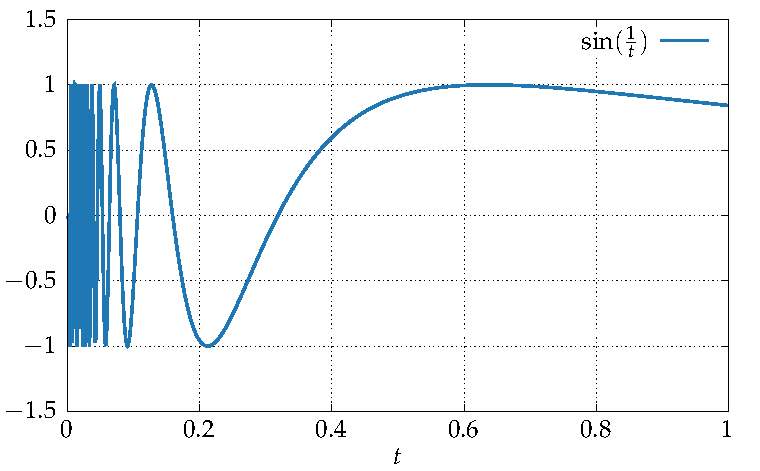
\includegraphics{gp_sininv.pdf}
  \caption{Curve of the function $f(t)=\sin(\frac{1}{t})$ from~\cref{ex:sininv}.}
  \label{fig:sininv}
\end{figure}
Finally, we show that the one-sided limits of the derivative of piecewise smooth functions
can be calculated with the usual limits:
\begin{proposition}
  \label{prop:oneside-der}
  Let $f$ be a piecewise smooth function on $[a,b]$, and let $t_0\in(a,b)$. The one-sided
  limits of $f'$ are given by the following limits
  \begin{equation}
    f'(t_0^-)=\lim_{\substack{h\to0\\h>0}}\frac{f(t_0^-)-f(t_0-h)}{h}
    \qquad\text{and}\qquad
    f'(t_0^+)=\lim_{\substack{h\to0\\h>0}}\frac{f(t_0+h)-f(t_0^+)}{h}
  \end{equation}
\end{proposition}
\begin{proof}
  Let $h>0$ small enough such that $t_0-h\in(a,b)$, and such that $f$ is continuously
  differentiable on $(t_0-h,t_0)$. Additionally, using condition (PC3)
  of~\cref{def:pw-cont}, $f$ restricted to $(t_0-h,t_0)$ can be extended to a continuous
  function on $[t_0-h,t_0]$ which take the value $f(t_0^-)$ in $t_0$. According to the
  mean value theorem, there exists $c_h$ in $(t_0-h,t_0)$ such that
  \begin{equation}
    f'(c_h)=\frac{f(t_0^-)-f(t_0-h)}{h}\,.
  \end{equation}
  Since $t_0-h<c_h<t_0$, then clearly $c_h\to t_0$ for $h\to 0$ with $h>0$, therefore
  \begin{equation}
    \lim_{\substack{h\to0\\h>0}}f'(c_h)=f'(t_0^-)
    =\lim_{\substack{h\to0\\h>0}}\frac{f(t_0^-)-f(t_0-h)}{h}\,.
  \end{equation}
  This proves the proposition for the left limit of $f'$. The right limit can be
  identically proven by considering the mean value theorem on a small interval
  $[t_0,t_0+h]$.
\end{proof}

%%%%%%%%%%%%%%%%%%%%%%%%%%%%%%%%%%%%%%%%%%%%%%%%%%%%%%%%%%%%%%%%%%%%%%%%%%%%%%%%%%%%%%%%%%
\section{Partial Fourier sums}
In this section, we formalise the generalisation of the
coefficients~\cref{eq:series-an-intro,eq:series-bn-intro,eq:series-cn-intro} mentioned in
the introduction to this section, as well as the associated trigonometric polynomials.
%.........................................................................................
\subsection{Fourier coefficients}
\begin{definition}
  \label{def:fourier-coef}
  Let $f$ be a piecewise smooth $\tau$-periodic function. We call \emph{cosine},
  \emph{sine}, and \emph{complex Fourier coefficients} the sequences
  \begin{align}
    a_n(f)&=\frac{2}{\tau}\braket{f,\cw(n\omega)}
    =\frac{2}{\tau}\int_0^{\tau}\diff t\,f(t)\cos(2\pi n\omega t)\,,\\
    b_n(f)&=\frac{2}{\tau}\braket{f,\sw(n\omega)}
    =\frac{2}{\tau}\int_0^{\tau}\diff t\,f(t)\sin(2\pi n\omega t)\,,\\
    c_n(f)&=\frac{1}{\tau}\braket{f,\ew(n\omega)}
    =\frac{1}{\tau}\int_0^{\tau}\diff t\,f(t)\,e^{-2\pi i n\omega t}\,,
  \end{align}
  respectively, where $n\in\mathbb{Z}$ and $\omega=\frac{1}{\tau}$.
\end{definition}
\begin{definition}
  \label{def:fourier-partial}
  Let $f$ be a piecewise smooth $\tau$-periodic function. For any integer $N\geq 0$, we
  call \emph{partial Fourier sum} of degree $N$ the trigonometric polynomial defined by
  \begin{equation}
    s_N(f)=\frac{a_0(f)}{2}+\sum_{n=1}^N[a_n(f)\cw(n\omega)+b_n(f)\sw(n\omega)]=
    \sum_{n=-N}^{N}c_n(f)\ew(n\omega)\,,
  \end{equation}
  where $\omega=\frac{1}{\tau}$.
\end{definition}
Since we aim at studying the convergence of Fourier sums for $N\to+\infty$, an important
question is the asymptotic behaviour of Fourier coefficients for $n\to+\infty$, discussed
in the next section.
%.........................................................................................
\subsection{Riemann-Lebesgue lemma}
For a fairly general class of functions, it can be shown that these coefficients converge
to $0$ for $n\to+\infty$. This is a crucial result in Fourier analysis generally called
the~\emph{Riemann-Lebesgue lemma}, and a necessary condition for the convergence of
Fourier series. We prove this result below for piecewise continuous functions on compact
intervals.
\begin{theorem}[Riemann-Lebesgue lemma]
  \label{thm:rl}
  Let $f$ be a piecewise continuous function on a compact interval $[a,b]$. We have the
  following limit
  \begin{equation}
    \lim_{k\to+\infty}\int_a^b\diff t\, f(t)\sin(kt)=0
  \end{equation}
\end{theorem}
\begin{proof}
  The proof of this theorem is rather abstract and technical, but it is based on a fairly
  intuitive idea. A first observation one can make is that the Riemann-Lebesgue lemma is
  easily demonstrated for constant functions. Indeed, for any constant $A\in\mathbb{R}$
  \begin{equation}
    \int_a^b\diff t\,A\sin(kt)=\frac{A}{k}\,[\cos(ka)-\cos(kb)]\,.
    \label{eq:rl-const}
  \end{equation}
  Then $|\cos(ka)-\cos(kb)|<2$ for all $k\in\mathbb{R}$, so the integral above clearly
  converges to $0$ for $k\to+\infty$. In the general case where $f$ is piecewise
  continuous, $f$ is an assembly of bounded continuous functions. Such functions can be
  approximated arbitrarily well by piecewise constant functions, similarly to what is done
  when approximating an integral with rectangles. With such a construction, the simple
  example above with constant functions is then all that is needed to prove the theorem.
  Let us proceed with justifying this approach in details.

  Reusing the notation of~\cref{def:pw-cont}, we have
  \begin{equation}
    \int_a^b\diff t\, f(t)\sin(kt)
    =\sum_{n=0}^{N}\int_{t_n}^{t_{n+1}}\diff t\, f(t)\sin(kt)\,.
    \label{eq:pw-int}
  \end{equation}
  The function $f$ is piecewise continuous, so according to condition (PC1)
  of~\cref{def:pw-cont}, for a given integer $n$ such that $0\leq n<N$, $f$ is continuous
  on $(t_n,t_{n+1})$. Additionally, conditions (PC2) and (PC3) imply that $f$ admits
  finite right and left limits in $t_n$ and $t_{n+1}$, respectively. Therefore, the
  restriction of $f$ to $(t_n,t_{n+1})$ can be extended to a continuous function on the
  compact interval $[t_n,t_{n+1}]$. Now, continuous functions on compact intervals are
  uniformly continuous, \ie for all $\epsilon>0$, there exists $\delta>0$ such that for
  all pairs $x,y$ in $[t_n,t_{n+1}]$, $|x-y|<\delta$ implies that $|f(x)-f(y)|<\epsilon$.
  Let us subdivide the interval $[t_n,t_{n+1}]$ into $M$ points
  $r_0=t_n<r_1<\dots<r_{M-1}<r_M=t_{n+1}$ such that for all $m$ with $0\leq m<M$,
  $|r_{n+1}-r_n|<\eta$. We then define the piecewise constant function $g$ equal to the
  constant $f(r_m)$ on $[r_m,r_{m+1})$, and $g(r_N)=f(r_{N-1})$. For a given point
  $t\in(t_n,t_{n+1})$, there exists $m$ such that $t\in[r_m,r_{m+1})$, and therefore
  \begin{equation}
    |f(t)-g(t)|=|f(t)-f(r_m)|<\epsilon\,,
  \end{equation}
  since by construction $|t-r_m|<\delta$. We can now write
  \begin{equation}
    \int_{t_n}^{t_{n+1}}\diff t\, f(t)\sin(kt)
    =\int_{t_n}^{t_{n+1}}\diff t\, [f(t)-g(t)]\sin(kt)
    +\int_{t_n}^{t_{n+1}}\diff t\,g(t)\sin(kt)\,.
  \end{equation}
  The integral of $g$ above can be dealt with easily, as anticipated in the introduction
  of the proof, explicitly
  \begin{equation}
    \int_{t_n}^{t_{n+1}}\diff t\,g(t)\sin(kt)
    =\frac{1}{k}\sum_{m=0}^{M-1}f(r_m)[\cos(kr_m)-\cos(kr_{m+1})]\,,
  \end{equation}
  so
  \begin{equation}
    \lim_{k\to0}\,\int_{t_n}^{t_{n+1}}\diff t\,g(t)\sin(kt)=0\,.
    \label{eq:rl-intg}
  \end{equation}
  Now, using the triangle inequality,
  \begin{equation}
    \left|\int_{t_n}^{t_{n+1}}\diff t\, [f(t)-g(t)]\sin(kt)\right|<
    \int_{t_n}^{t_{n+1}}\diff t\, |f(t)-g(t)|<(t_{n+1}-t_n)\epsilon\,.
  \end{equation}
  Since $\epsilon$ can be chosen arbitrarily small, the inequality above implies that
  \begin{equation}
    \lim_{k\to0}\,\int_{t_n}^{t_{n+1}}\diff t\, [f(t)-g(t)]\sin(kt)=0\,.
    \label{eq:rl-intfmg}
  \end{equation}
  Combining~\cref{eq:rl-intg,eq:rl-intfmg}, we just proved that every term in the sum
  in~\cref{eq:pw-int} converges to $0$ for $k\to+\infty$, which demonstrates the theorem.
\end{proof}
\begin{figure}[t]
  \centering
  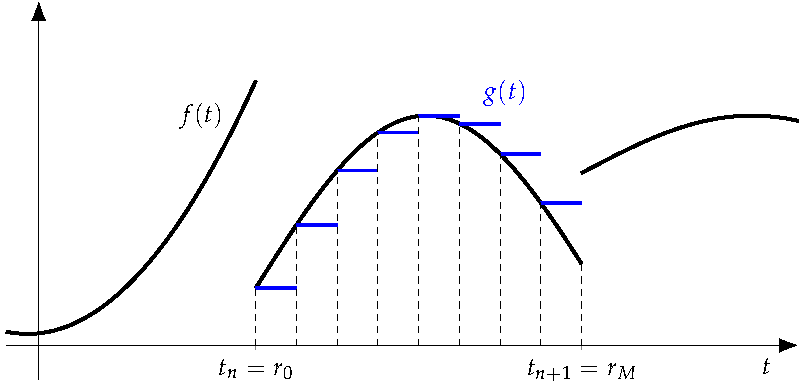
\includegraphics{tikz_rl.pdf}
  \caption{Illustration of the construction used in the proof of~\cref{thm:rl}
    (Riemann-Lebesgue lemma). The black curve represents an arbitrary piecewise continuous
    function, with visible jump discontinuities at $t_n$ and $t_{n+1}$. The blue lines
    represent a piecewise constant approximation $g$ of $f$ on the interval
  $[t_n,t_{n+1}]$, as defined in the proof of~\cref{thm:rl}}
  \label{fig:rl}
\end{figure}
\begin{corollary}
  Let $f$ be a function on $\mathbb{R}$ piecewise smooth on a compact interval $[a,b]$. We
  have the following limits
  \begin{align}
    \lim_{k\to+\infty}\int_a^b\diff t\, f(t)\cos(kt)&=0\,,\\
    \lim_{k\to+\infty}\int_a^b\diff t\, f(t)\,e^{ikt}=0
  \end{align}
\end{corollary}
\begin{proof}
  One can inspect the proof of~\cref{thm:rl} and notice that the only dependency on the
  $\sin(kt)$ weight in the integral comes from~\cref{eq:rl-const}. So it is sufficient to
  just repeat that step for the cosine function. We have
  \begin{equation}
    \int_a^b\diff t\, f(t)\cos(kt)=\frac{1}{k}[\sin(bk)-\sin(ak)]\,,
  \end{equation}
  and since $|\sin(bk)-\sin(ak)|<2$ for all $k\in\mathbb{R}$, the integral above vanishes
  for $k\to+\infty$. A similar argument can be made for the complex exponential, although
  one can also notice that it is now a trivial consequence the equality
  \begin{equation}
    \int_a^b\diff t\, f(t)\,e^{ikt}
    =\int_a^b\diff t\, f(t)\cos(kt)+i\int_a^b\diff t\, f(t)\sin(kt)\,.
  \end{equation}
\end{proof}
\begin{corollary}
  Let $f$ be a piecewise smooth $\tau$-periodic function. All the Fourier coefficients of
  $f$ converge to $0$, explicitly
  \begin{equation}
    \lim_{n\to+\infty}a_n(f)=\lim_{n\to+\infty}b_n(f)=\lim_{n\to+\infty}c_n(f)=0\,.
  \end{equation}
\end{corollary}
\begin{proof}
  This is a trivial consequence of the Riemann-Lebesgue lemma applied
  to~\cref{def:fourier-coef}.
\end{proof}
%.........................................................................................
\subsection{Dirichlet kernel}
In this section, we discuss a special function called the \emph{Dirichlet kernel}. This
function allows to write the partial Fourier sums as an integral (and as we will see in
later chapters, a convolution product), which is often used in combination with the
Riemann-Lebesgue lemma to demonstrate theorems on the convergence of Fourier series.
\begin{definition}
  We call~\emph{Dirichlet kernel} of degree $N$ the trigonometric polynomial defined by
  \begin{equation}
    D_N(x)=\sum_{n=-N}^{N}e^{inx}\,,\label{eq:dk-def}
  \end{equation}
  for any real number $x$. The Dirichlet kernel is by construction even and periodic with
  fundamental period $2\pi$.
\end{definition}
The Dirichlet kernel can in fact be expressed as a simple ratio of sine functions as
discussed in the result below.
\begin{proposition}
  \label{prop:dirichlet-id}
  For all $x\in\mathbb{R}$, and all $N\in\mathbb{N}$, we have
  \begin{equation}
    D_N(x)=1+2\sum_{n=1}^{N}\cos(nx)=\frac{\sin[(N+\frac{1}{2})x]}{\sin(\frac{x}{2})}\,.
    \label{eq:dk-sinratio}
  \end{equation}
\end{proposition}
\begin{proof}
  We start by defining the complex number $z$ by
  \begin{equation}
    z=\sum_{n=0}^Ne^{inx}\,.
  \end{equation}
  The Dirichlet kernel can then be written as follows:
  \begin{equation}
    D_N(x)=(z-1)^*+z=z^*+z-1=2\Re(z)-1=1+2\sum_{n=1}^{N}\cos(nx)\,,\label{eq:dk-z}
  \end{equation}
  which proves the first equality in~\cref{eq:dk-sinratio}. Since $e^{inx}=(e^{ix})^n$, we
  can simplify $z$ using a geometric sum:
  \begin{equation}
    z=\frac{e^{i(N+1)x}-1}{e^{ix}-1}\,.\label{eq:dk-geosum}
  \end{equation}
  We now have to compute the real part of $z$, let us start by rewriting the equation
  above to have a real denominator:
  \begin{equation}
    z=e^{-i\frac{x}{2}}\frac{e^{i(N+1)x}-1}{e^{i\frac{x}{2}}-e^{-i\frac{x}{2}}}
    =\frac{e^{i(N+\frac12)x}-e^{-i\frac{x}{2}}}{2i\sin(\frac{x}{2})}
    =-\frac{i}{2}\frac{e^{i(N+\frac12)x}-e^{-i\frac{x}{2}}}{\sin(\frac{x}{2})}\,,
  \end{equation}
  which has the real part
  \begin{equation}
    \Re(z)=\frac12\frac{\Im[e^{i(N+\frac12)x}]-\Im(e^{-i\frac{x}{2}})}{\sin(\frac{x}{2})}
    =\frac12\frac{\sin[(N+\frac{1}{2})x]}{\sin(\frac{x}{2})}+1\,.
  \end{equation}
  Substituting the last equation into~\cref{eq:dk-z} proves the proposition.
\end{proof}
\begin{proposition}
  \label{prop:dk-int}
  The Dirichlet kernel has the following integral on $[0,2\pi]$ for all $N\in\mathbb{N}$:
  \begin{equation}
    \int_0^{2\pi}\diff x\,D_N(x)=2\pi\,.
  \end{equation}
\end{proposition}
\begin{proof}
  Using~\cref{thm:orth-complex} with $m=0$ and $\tau=2\pi$, we obtain
  \begin{equation}
    \int_{0}^{2\pi}\diff x\,e^{inx}=2\pi\,\delta_{n0}\,,
  \end{equation}
  which substituted into~\cref{eq:dk-def} directly proves the proposition.
\end{proof}
We now formulate the main theorem on the integral representation of partial Fourier sums.
\begin{theorem}
  \label{thm:fourier-dk-rep}
  Let $f$ be a piecewise smooth $\tau$-periodic function. For all $N\in\mathbb{N}$, the
  partial Fourier sum of $f$ has the following integral representation:
  \begin{equation}
    s_N(f)(t)=\frac{1}{\tau}\int_0^{\tau}\diff u\,f(u)\,D_N[2\pi\omega(t-u)]\,.
  \end{equation}
\end{theorem}
\begin{proof}
  Using~\cref{def:fourier-coef,def:fourier-partial}, the partial Fourier sum $s_N(f)$ is
  given by
  \begin{equation}
    s_N(f)(t)=\frac{1}{\tau}\sum_{n=-N}^{N}e^{2\pi i n\omega t}
    \int_0^\tau\diff u\,f(u)e^{-2\pi i n\omega u}\,.
  \end{equation}
  Since the sum above is finite, we can exchange the sum and the integral to obtain
  \begin{equation}
    s_N(f)(t)=\frac{1}{\tau}\int_0^\tau\diff u\,f(u)\sum_{n=-N}^{N}e^{2\pi i n\omega (t-u)}\,.
  \end{equation}
  Finally, using the definition of the Dirichlet kernel~\cref{eq:dk-def} proves the
  theorem.
\end{proof}
%%%%%%%%%%%%%%%%%%%%%%%%%%%%%%%%%%%%%%%%%%%%%%%%%%%%%%%%%%%%%%%%%%%%%%%%%%%%%%%%%%%%%%%%%%
\section{Convergence of the Fourier expansion}
Using results from the previous section, we are now ready to discuss in details the
convergence of Fourier series. We start by discussing pointwise convergence, in a context
close to the original work of Peter Gustav Lejeune Dirichlet and Camille Jordan in the
second half of the 19\textsuperscript{th}, who brought stronger mathematical foundations
to the pioneering work of Fourier. We will then discuss the much stronger case of uniform
convergence, and conclude the section with the Gibbs phenomenon, which describes important
practical consequences of Fourier series which fail to converge uniformly.
%-----------------------------------------------------------------------------------------
\subsection{Pointwise convergence}
The theorem below can be considered as the main result of this chapter. It states that for
piecewise smooth periodic functions, the Fourier series converges at every point to the
average of the left and right limits. The essence of this theorem is that the Fourier
series does converge back to a given piecewise smooth periodic function, expect perhaps at
a finite number of points of jump discontinuity.
\begin{theorem}
  \label{thm:fourier-pt}
  Let $f$ be a $\tau$-periodic function which is piecewise smooth on $[0,\tau]$. For all
  $t\in\mathbb{R}$, the Fourier series for $f(t)$ converges with the following limit
  \begin{equation}
    \sumz{n}c_n(f)\,e^{2\pi i \omega nt}=\lim_{N\to+\infty}s_N(f)(t)
    =\frac{f(t^-)+f(t^+)}{2}\,.
  \end{equation}
  In particular, the Fourier series converges to $f(t)$ if $f$ is continuous in $t$.
\end{theorem}
\begin{proof}
  Let $t$ be a point in $[0,\tau]$. Using~\cref{thm:fourier-dk-rep}, we can write the
  partial Fourier sum $s_N(f)$ at the point $t$ as
  \begin{equation}
    s_N(f)(t)=\frac{1}{\tau}\int_{-\frac{\tau}{2}}^{\frac{\tau}{2}}\diff u\,
    f(u)\,D_N[2\pi\omega(t-u)]\,,
  \end{equation}
  where $\omega=\frac{1}{\tau}$, and the integration domain was shifted to
  $(-\frac{\tau}{2},\frac{\tau}{2})$, which is allowed by the $\tau$-periodicity of the
  integrand. We additionally perform the change of variable $u\mapsto t-u$ to obtain
  \begin{equation}
    s_N(f)(t)=\frac{1}{\tau}\int_{-\frac{\tau}{2}}^{\frac{\tau}{2}}\diff u\,
    f(t-u)\,D_N(2\pi\omega u)\,.
  \end{equation}
  Now, using~\cref{prop:dk-int}, we get
  \begin{equation}
    \int_{-\frac{\tau}{2}}^{\frac{\tau}{2}}\diff u\,D_N(2\pi\omega u)
    =\frac{\tau}{2\pi}\int_{-\pi}^{\pi}\diff x\,D_N(x)=
    \frac{\tau}{2\pi}\int_{0}^{2\pi}\diff x\,D_N(x)=\tau\,,
    \label{eq:fthm-partsum}
  \end{equation}
  where we used the change of variable $x=2\pi\omega u$, as well as the $2\pi$-periodicity
  of the Dirichlet kernel. Similarly, since $D_N(x)$ is even, we can write
  \begin{equation}
    \int_{0}^{\frac{\tau}{2}}\diff u\,D_N(2\pi\omega u)
    =\int_{-\frac{\tau}{2}}^{0}\diff u\,D_N(2\pi\omega u)=\frac{\tau}{2}\,.
  \end{equation}
  Since $f(t^-)$ and $f(t^+)$ are just constants, we can write
  \begin{align}
    \frac{f(t^-)}{2}&=\frac{1}{\tau}\int_{0}^{\frac{\tau}{2}}\diff u\,
    f(t^-)D_N(2\pi\omega u)\,,
    \label{eq:fthm-tmint}\\
    \frac{f(t^+)}{2}&=\frac{1}{\tau}\int_{-\frac{\tau}{2}}^{0}\diff u\,
    f(t^+)D_N(2\pi\omega u)\,.
    \label{eq:fthm-tpint}
  \end{align}
  We consider the two following integrals
  \begin{align}
    I^-_N&=\frac{1}{\tau}\int_{0}^{\frac{\tau}{2}}\diff u\,
    [f(t-u)-f(t^-)]D_N(2\pi\omega u)\,,\\
    I^+_N&=\frac{1}{\tau}\int_{-\frac{\tau}{2}}^{0}\diff u\,
    [f(t-u)-f(t^+)]D_N(2\pi\omega u)\,.
  \end{align}
  Using~\cref{eq:fthm-partsum,eq:fthm-tmint,eq:fthm-tpint}, we get
  \begin{equation}
    I^-_N+I^+_N=s_N(f)(t)-\frac{f(t^-)+f(t^+)}{2}\,.
    \label{eq:fourier-imip}
  \end{equation}
  Therefore, if we can show that $I^-_N$ and $I^+_N$ converge to $0$ for $N\to+\infty$,
  then the theorem is proven. Let us start by discussing $I^-_N$.
  Using~\cref{prop:dirichlet-id}, we can write
  \begin{equation}
    I^-_N=\frac{1}{\tau}\int_{0}^{\frac{\tau}{2}}\diff u\,
    \varphi^-(u)\sin\left[\left(N+\frac{1}{2}\right)2\pi\omega u\right]\,,
  \end{equation}
  where $\varphi^-$ is the function defined on all $u\in(0,\frac{\tau}{2})$ by
  \begin{equation}
    \varphi^-(u)=\frac{f(t-u)-f(t^-)}{\sin(\pi\omega u)}
    =\frac{f(t-u)-f(t^-)}{u}\frac{u}{\sin(\pi\omega u)}\,.
  \end{equation}
  If we can prove that $\varphi^-$ is piecewise continuous on
  $\smash{[0,\frac{\tau}{2}]}$, then $I^-_N$ converging to zero for $N\to+\infty$ is a
  direct consequence of the Riemann-Lebesgue lemma. Since $\sin(\pi\omega u)\neq 0$ for
  all $u\in\smash{(0,\frac{\tau}{2}]}$, and $f$ is piecewise smooth, the formula above
  clearly satisfies conditions (PC1) and (PC2) of~\cref{def:pw-cont}. However, it has an
  apparent singularity at $u=0$ that needs to be discussed for (PC3) to hold. For $u\to
  0$, $\sin(\pi\omega u)=\pi\omega u+\mathcal{O}(u^2)$ and therefore
  \begin{equation}
    \lim_{u\to 0}\,\frac{u}{\sin(\pi\omega u)}=\frac{1}{\pi\omega}\,.
  \end{equation}
  Then, using~\cref{prop:oneside-der}, we obtain
  \begin{equation}
    \lim_{\substack{u\to0\\u>0}}\varphi^-(u)=-\frac{f'(t^-)}{\pi\omega}\,,
  \end{equation}
  So $\varphi^-$ has a well-defined right limit for $u\to 0$, condition (PC3) is
  satisfied, $\varphi^-$ is piecewise continuous on $\smash{[0,\frac{\tau}{2}]}$,
  and~\cref{thm:rl} implies that
  \begin{equation}
    \lim_{N\to+\infty}I^-_N=0\,.
  \end{equation}
  We similarly write $I_N^+$ as
  \begin{equation}
    I^+_N=\frac{1}{\tau}\int_{-\frac{\tau}{2}}^{0}\diff u\,
    \varphi^+(u)\sin\left[\left(N+\frac{1}{2}\right)2\pi\omega u\right]\,,
  \end{equation}
  where
  \begin{equation}
    \varphi^+(u)=\frac{f(t-u)-f(t^+)}{\sin(\pi\omega u)}\,.
  \end{equation}
  As above, the limit
  \begin{equation}
    \lim_{\substack{u\to0\\u<0}}\varphi^+(u)=\frac{f'(t^+)}{\pi\omega}
  \end{equation}
  shows that $\varphi^+$ is piecewise continuous on $\smash{[-\frac{\tau}{2},0]}$, and
  therefore
  \begin{equation}
    \lim_{N\to+\infty}I^+_N=0\,.
  \end{equation}
  Coming back to~\cref{eq:fourier-imip}, the theorem is proven.
\end{proof}
\begin{example}
  The Fourier series of the square wave $\sq$ defined in~\cref{eq:wave-square} converges
  to the function
  \begin{equation}
    \sumz{n}c_n(\sq)\,e^{2\pi i \omega nt}=
    \begin{cases}
      1&\text{if}~0<t<\frac{1}{2}\\
      -1&\text{if}~\frac{1}{2}<t<-1\\
      \frac{1}{2}&\text{if}~t=0,\frac{1}{2},1
    \end{cases}\,,
  \end{equation}
  where it is understood that these values are repeated on every period. This limit is
  identical to the square wave except at the points of discontinuity where it takes the
  value $\frac{1}{2}$.
\end{example}
%-----------------------------------------------------------------------------------------
\subsection{Convergence in mean square and Parseval's theorem}
Another useful form of convergence for sequences of functions is the \emph{convergence in mean square}, also called \emph{$L^2$ convergence}, based on the functional norm introduced in~\cref{sec:ew-orth}. In all this section, we will work with square-integrable $\tau$-periodic functions. Such a function $f$ is defined by requiring that $|f|^2$ has a defined finite integral on $[0,\tau]$. This is the general class of functions for which the dot product is well-defined, which we will admit here. In particular, all piecewise smooth functions are square-integrable.
\begin{definition}
  Let $f$ be a $\tau$-periodic square-integrable function. A sequence of $\tau$-periodic square-integrable functions $f_n$ is said to converge to $f$ \emph{in mean} if
  \begin{equation}
    \lim_{n\to+\infty}\|f-f_n\|=0\,.
  \end{equation}
\end{definition}
This type of convergence is useful because the norm is related to the dot product of functions,
and as we saw in the previous chapter, the orthogonality of elementary waves. However, it is important to notice that this is a rather weak form of convergence, and without further assumptions it does not generally imply pointwise or uniform convergence.

We now generalise some results of~\cref{sec:ew-orth}, which we will then use to prove that Fourier series generally converge in mean square. Firstly, it is not too difficult to
show that the norm of a partial Fourier sum is always smaller than the norm of the associated function,
an important result known as \emph{Bessel's inequality}.
\begin{theorem}[Bessel's inequality]
  \label{thm:bessel}
  Let $f$ be a piecewise smooth $\tau$-periodic function. The series over $n\in\mathbb{Z}$
  with summand $|c_n(f)|^2$ converges, and one has the inequality
  \begin{equation}
    \tau\sumz{n}|c_n(f)|^2\leq\|f\|^2\,.
  \end{equation}
\end{theorem}
\begin{proof}
  We consider the norm of the difference between $f$ and its partial Fourier sum
  \begin{equation}
    \Delta_N=\|f-s_N(f)\|^2\,,
  \end{equation}
  where $N$ is some positive integer. By construction, $\Delta_N\geq 0$ for all $N>0$.
  Additionally, $\Delta_N$ can be expanded as
  \begin{align}
    \Delta_N&=\braket{f-s_N(f),f-s_N(f)}\\
    &=\|f\|^2+\|s_N(f)\|^2-2\Re[\braket{f,s_N(f)}]\,.\label{eq:bessel-l2err}
  \end{align}
  Furthermore,
  \begin{align}
    \braket{f,s_N(f)}&=\Braket{f,\sum_{n=-N}^{N}c_n(f)\ew(n\omega)}\\
    &=\sum_{n=-N}^{N}c_n(f)^*\braket{f,\ew(n\omega)}\\
    &=\tau\sum_{n=-N}^{N}|c_n(f)|^2\,.
  \end{align}
  Using Parseval's theorem for trigonometric polynomials (\cref{thm:trigp-parseval}), the result
  above implies that $\braket{f,s_N(f)}=\|s_N(f)\|^2$. Substituting this expression back into
  \cref{eq:bessel-l2err}, we get
  \begin{equation}
    \Delta_N=\|f\|^2-\|s_N(f)\|^2\,,
  \end{equation}
  and since $\Delta_N\geq 0$,
  \begin{equation}
    \forall N>0,\quad \|s_N(f)\|^2=\tau\sum_{n=-N}^{N}|c_n(f)|^2\leq \|f\|^2\,.
  \end{equation}
  $\|s_N(f)\|^2$ is a sum of positive numbers, and therefore a monotonous sequence in $N$. As per the inequality above, it is bounded by $\|f\|^2$ and therefore converges, which proves the theorem.
\end{proof}
In reality, this inequality is an equality, generalising~\cref{thm:trigp-parseval}. This is a much harder result to prove, and we will admit it here.
\begin{theorem}[Parseval]
  \label{thm:parseval}
  Let $f$ and $g$ be two square-integrable $\tau$-periodic functions. The following identities hold
  \begin{align}
    \braket{f,g}&=\tau\sumz{n}c_n(f)c_n(g)^*\,,
    \label{eq:fs-dot}\\
    \|f\|^2&=\tau\sumz{n}|c_n(f)|^2\,.
    \label{eq:fs-norm}
  \end{align}
\end{theorem}
For completeness, we provide below the Parseval theorem identities for the sine-cosine form
\begin{align}
  \braket{f,g}&=\tau\,\frac{a_0(f)a_0(g)^*}{4}
  +\frac{\tau}{2}\left\{\sumnp{n}[a_n(f)a_n(g)^*+b_n(f)b_n(g)^*]\right\}\,,\\
  \|f\|^2&=\tau\,\frac{|a_0(f)|^2}{4}+\frac{\tau}{2}\left\{\sumnp{n}[|a_n(f)|^2+|b_n(f)|^2]\right\}\,.
\end{align}
\begin{theorem}
  Let $f$ be a square-integrable $\tau$-periodic function. The Fourier series of $f$
  converges to $f$ in mean.
\end{theorem}
\begin{proof}
  We need to show that
  \begin{equation}
    \Delta_N =\|f-s_N(f)\|^2
  \end{equation}
  converges to $0$ for $N\to+\infty$. As already demonstrated in the proof of~\cref{thm:bessel},
  \begin{equation}
    \Delta_N =\|f\|^2-\tau\sum_{n=-N}^{N}|c_n(f)|^2\,.\label{eq:l2cvg-deltan}
  \end{equation}
  Using Parseval's theorem, we know that
  \begin{equation}
    \lim_{N\to+\infty}\tau\sum_{n=-N}^{N}|c_n(f)|^2=\|f\|^2\,,
  \end{equation}
  which applied to~\cref{eq:l2cvg-deltan} proves the theorem.
\end{proof}
The proof above is quite simple once one knows Parseval's theorem. In fact, Parseval's theorem
is truly the non-trivial property here, and it can be shown to be a necessary and sufficient condition
to the convergence in mean square. Proving Parseval's theorem it quite technical and out of the scope of this introductory course, however we will sketch the proof in the next section.
\subsection{Uniform convergence}
We start by reminding the definition of uniform convergence for a sequence of functions.
Essentially, such sequence is uniformly convergent if the distance to the limit can be
bounded independently of the point at which the function is evaluated, as formalised in
the definition below.
\begin{definition}
  A sequence of function $f_n$ is said to \emph{converge uniformly} to $f$ on a domain $D$
  if for all $\epsilon>0$, there exists $N\in\mathbb{N}$ such that
  \begin{equation}
    \forall n\geq N,\quad\forall x\in D,\quad|f_n(x)-f(x)|<\epsilon\,,
  \end{equation}
  which can equivalently be defined as the limit
  \begin{equation}
    \lim_{n\to+\infty}\,\sup_{x\in D}|f_n(x)-f(x)|=0\,.
  \end{equation}
\end{definition}
\begin{example}
  The sequence of functions defined by $\sin(t+\frac{1}{n})$ converges uniformly to
  $\sin(t)$ in the $n\to+\infty$ limit. Indeed,
  \begin{equation}
    \sin\left(t+\frac{1}{n}\right)-\sin(t)
    =2\sin\left(\frac{1}{2n}\right)\cos\left(t+\frac{1}{2n}\right)\,,
  \end{equation}
  therefore
  \begin{equation}
    \sup_{t\in\mathbb{R}}\left|\sin\left(t+\frac{1}{n}\right)
    -\sin(t)\right|=2\sin\left(\frac{1}{2n}\right)\,.
  \end{equation}
  The right-hand side of the equation above converges to $0$ for $n\to+\infty$, which
  proves the uniform convergence.
\end{example}
\begin{example}
  The sequence of functions defined by $t^n$ converges uniformly to $0$ on any interval of
  the form $[0,a]$ with $a<1$, but not on $[0,1)$. Indeed, for $t\in [0,1)$, clearly
  \begin{equation}
    \lim_{n\to+\infty}t^n=0\,,
  \end{equation}
  so $t^n$ converges pointwise to $0$ on $[0,1)$. Let $a\in(0,1)$, since $t^n$ is a
  positive, increasing function for $t>0$, we have
  \begin{equation}
    \sup_{t\in[0,a]}|t^n|=a^n\,,
  \end{equation}
  and since $a<1$,
  \begin{equation}
    \lim_{n\to+\infty}\sup_{t\in[0,a]}t^n=0\,,
  \end{equation}
  so $t^n$ converges uniformly to $0$ on $[0,a]$. However,
  \begin{equation}
    \sup_{t\in[0,1)}|t^n|=1\,,
  \end{equation}
  so $t^n$ does not converge uniformly to $0$ on $[0,1)$.
\end{example}
\begin{theorem}
  Let $f$ be a $\tau$-periodic function which is piecewise smooth and continuous on
  $[0,\tau]$. The Fourier series of $f$ converges uniformly to $f$.
\end{theorem}
\subsection{Gibbs phenomenon}
If a periodic function has a jump discontinuity, then its Fourier series cannot be
uniformly convergent. This generates irregularities around discontinuities where the
Fourier expansion tends to ``overshoot'' the function by approximately $9\%$ of the height
of the discontinuity. This effect is generally called the \emph{Gibbs phenomenon}, and is
a well known engineering issue when cutting data before computing its Fourier
coefficients. A key example of Gibbs phenomenon is the Fourier expansion of the square
wave.
\begin{lemma}
  \label{lem:gibbs-sq}
  The square wave Fourier series does not converge uniformly on $[0,1]$, and
  \begin{align}
    \lim_{N\to+\infty}\,s_N(\sq)\left(\frac12-\frac{1}{2N}\right)
    &=1+2\left(\frac{G'}{\pi}-\frac12\right)\,,\label{eq:gibbs-sq-left}\\
    \lim_{N\to+\infty}\,s_N(\sq)\left(\frac12+\frac{1}{2N}\right)
    &=-1-2\left(\frac{G'}{\pi}-\frac12\right)\,,
  \end{align}
  where $G'$ is the \emph{Wilbraham-Gibbs constant} given by
  \begin{equation}
    G'=\int_0^\pi\diff t\,\frac{\sin(t)}{t}\simeq1.851937052\dots\,.
  \end{equation}
\end{lemma}
\begin{proof}
  A guided proof is available as an exercise in Problem~\ref{gibbs}.
\end{proof}
\begin{figure}[t]
  \centering
  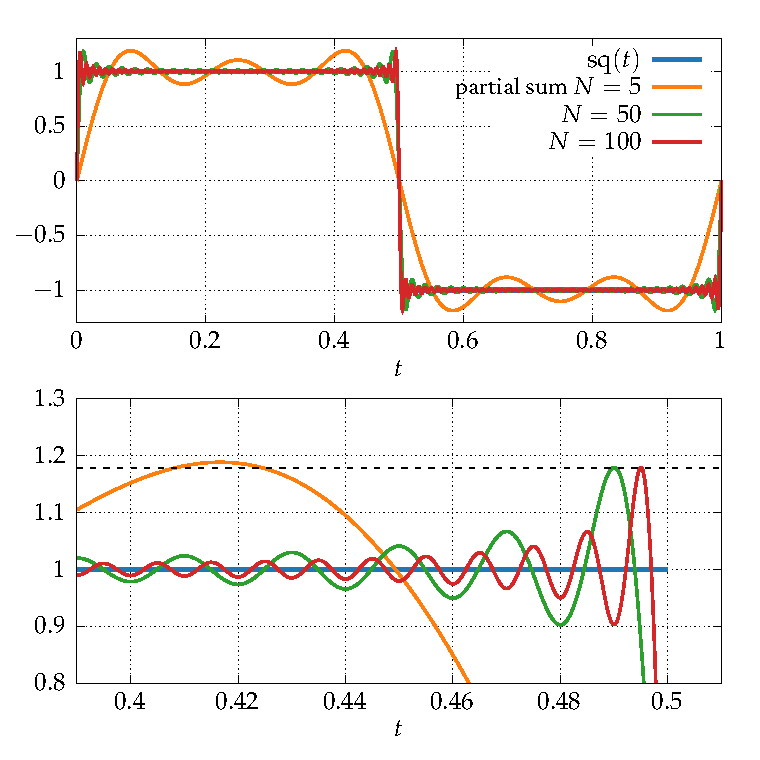
\includegraphics{gp_gibbs-sq.pdf}
  \caption{Gibbs phenomenon in the Fourier expansion of the square wave. The upper pane
    represents the square wave on one period, and its partial Fourier sum for various
    degrees. The lower pane is a zoom on the region close to the jump discontinuity at
  $t=\frac12$, and the dashed line is the excess predicted by~\cref{eq:gibbs-sq-left}.}
  \label{fig:gibbs-sq}
\end{figure}
The Fourier expansion of the square wave is illustrated in~\cref{fig:gibbs-sq}, where the
Gibbs phenomenon is clearly visible. The Gibbs phenomenon for the square wave can be
generalised to arbitrary discontinuous piecewise smooth functions, as summarised in the
theorem below.
\begin{theorem}[Gibbs phenomenon]
  Let be a $\tau$-periodic function which is piecewise smooth on $[0,\tau]$, which has a
  jump discontinuity of height $d$ at $t_0\in(0,\tau)$. Let $[a,b]$ be a sub-interval of
  $[0,\tau]$ such that $t_0\in(a,b)$, and $t_0$ is the only jump discontinuity of $f$ in
  $[a,b]$. The Fourier series of $f$ does not converge uniformly to $f$ on $[a,b]$, and
  \begin{align}
    \lim_{N\to+\infty}\,s_N(f)\left(t_0-\frac{\tau}{2N}\right)
    &=f(t_0^-)-d\left(\frac{G'}{\pi}-\frac12\right)\,,\\
    \lim_{N\to+\infty}\,s_N(f)\left(t_0+\frac{\tau}{2N}\right)
    &=f(t_0^+)+d\left(\frac{G'}{\pi}-\frac12\right)\,,
  \end{align}
  where $G'$ is the Wilbraham-Gibbs constant defined in~\cref{lem:gibbs-sq}.
\end{theorem}
%%%%%%%%%%%%%%%%%%%%%%%%%%%%%%%%%%%%%%%%%%%%%%%%%%%%%%%%%%%%%%%%%%%%%%%%%%%%%%%%%%%%%%%%%%
\section{Properties of Fourier coefficients}
%%%%%%%%%%%%%%%%%%%%%%%%%%%%%%%%%%%%%%%%%%%%%%%%%%%%%%%%%%%%%%%%%%%%%%%%%%%%%%%%%%%%%%%%%%
\section{Multidimensional Fourier series}

\chapter{Fourier transform}
% !TEX root = ../waves.tex
%%%%%%%%%%%%%%%%%%%%%%%%%%%%%%%%%%%%%%%%%%%%%%%%%%%%%%%%%%%%%%%%%%%%%%%%%%%%%%%%%%%%%%%%%%
%\section{Definition of the Fourier transform}
%%%%%%%%%%%%%%%%%%%%%%%%%%%%%%%%%%%%%%%%%%%%%%%%%%%%%%%%%%%%%%%%%%%%%%%%%%%%%%%%%%%%%%%%%%
%\section{Properties of the Fourier transform}
%%%%%%%%%%%%%%%%%%%%%%%%%%%%%%%%%%%%%%%%%%%%%%%%%%%%%%%%%%%%%%%%%%%%%%%%%%%%%%%%%%%%%%%%%%
%\section{The Dirac delta distribution}
%%%%%%%%%%%%%%%%%%%%%%%%%%%%%%%%%%%%%%%%%%%%%%%%%%%%%%%%%%%%%%%%%%%%%%%%%%%%%%%%%%%%%%%%%%
%\section{The convolution theorem}
%%%%%%%%%%%%%%%%%%%%%%%%%%%%%%%%%%%%%%%%%%%%%%%%%%%%%%%%%%%%%%%%%%%%%%%%%%%%%%%%%%%%%%%%%%
%\section{Diagonalisation of differential operators}
\chapter{Applications}
% !TEX root = ../waves.tex
%%%%%%%%%%%%%%%%%%%%%%%%%%%%%%%%%%%%%%%%%%%%%%%%%%%%%%%%%%%%%%%%%%%%%%%%%%%%%%%%%%%%%%%%%%
\section{Solving partial differential equations}
%%%%%%%%%%%%%%%%%%%%%%%%%%%%%%%%%%%%%%%%%%%%%%%%%%%%%%%%%%%%%%%%%%%%%%%%%%%%%%%%%%%%%%%%%%
\section{Linear time-invariant systems}
%%%%%%%%%%%%%%%%%%%%%%%%%%%%%%%%%%%%%%%%%%%%%%%%%%%%%%%%%%%%%%%%%%%%%%%%%%%%%
% \bibliographystyle{apsrev4-2}
% \bibliography{BIB}
\end{document}
